\documentclass[12pt,a4paper]{IEEEtran}
\usepackage[margin=0.65in]{geometry}
\usepackage[affil-it]{authblk}
\usepackage{graphicx}
\usepackage[table,xcdraw]{xcolor}
\usepackage{caption}
\usepackage{subcaption}
\usepackage{float}
\usepackage{hyperref}
\usepackage{relsize}
\usepackage{textcomp}
\usepackage{kbordermatrix,amsmath}
{
	%	\theoremstyle{plain}
	\newtheorem{assumption}{Assumption}
}
\usepackage[most]{tcolorbox}
\tcbset{textmarker/.style={%
		enhanced,
		parbox=false,boxrule=0mm,boxsep=0mm,arc=0mm,
		outer arc=0mm,left=6mm,right=3mm,top=7pt,bottom=7pt,
		toptitle=1mm,bottomtitle=1mm}}

\newtcolorbox{importantBox}{textmarker,
	borderline west={6pt}{0pt}{red},
	colback=red!10!white}

\newcommand{\important}[1]{\begin{importantBox} \textbf{Important:} #1 \end{importantBox}}
\newcommand{\magn}[1]{\Vert{#1}\Vert}
\newcommand{\card}[1]{\vert{#1}\vert}
%\newcommand{\vbb}[2]{\vec{#1#2}}
\newcommand{\vbb}[2]{#2-#1}
%\renewcommand{\vec}[1]{\overrightarrow{#1}}
\newcommand{\pangle}{\mathit{\alpha}}
\newcommand{\leqaz}[3]{#2 \leq_{\pangle_#1} #3}
\newcommand{\angleordered}[2]{\langle #2 \rangle_{\leqaz{#1}{}{}}}
\newcommand{\prm}{\mathsf{prm}}
\newcommand{\kc}{\mathit{k_c}}
\newcommand{\kr}{\mathit{k_r}}
\newcommand{\kd}{\mathit{k_d}}
\newcommand{\kg}{\mathit{k_g}}
\newcommand{\ko}{\mathit{k_o}}
\newcommand{\rb}{\mathit{R}}
\newcommand{\rgf}{\mathit{rgf}}
\title{A Novel Relationship-based Approach to Swarm Coordination.}
\author[*]{Neil Eliot}
\author[ ]{David Kendall}
\author[ ]{Michael Brockway}
\author[ ]{Paul Oman}
\author[ ]{Ahmed Bouridane}
\affil[ ] {Department of Computer Sciences, Northumbria University}
\affil[*] {Corresponding author: Dr Neil Eliot, neil.eliot@northumbria.ac.uk}
\date{\today}


\begin{document}
\maketitle

\begin{abstract}
Most of the current models for swarm coordination are based upon fixed (single value) potential fields. This paper presents a new novel approach to swarm coordination which is relationship-based. The new technique allows useful emergent behaviours to be created that improve the structure of a swarm and make it applicable to specific applications such as reconnaissance where a high density swarm frontier may be required or a reduced perimeter density may be required at the frontier. The model is dependant upon perimeter identification. Using an agent's perimeter status alternative controlling dynamics can be induced. The movement is modified using three arrays that are indexed by the agent's status. The agent's vector calculations are modified by these array entries to produce the final movement vector. The results section of this paper demonstrates how the new model can implement behaviours such as packed and expanded perimeters to emerge for a random swarm deployment and how the new model can still operate as the traditional single value potential field model.
\end{abstract}

\section{Introduction}
When cohesion and repulsion field effects (sometimes referred to as potential fields~\cite{BAF:06,eliot2018metric,VG:05,SW:03,Son2017,liang2019swarm}) are used to create a swarming effect, the stable structures that develop are limited to either straight edges or partial lattices \cite{eliot2017methods}. The maintenance of a well-structured swarm is crucial to effective deployment for applications such as reconnaissance or artificial pollination, where `blind spots' are best eliminated \cite{elamvazhuthi2015optimal}, and containment, where the swarm is used to surround an object or region \cite{cao2012distributed}. Over time swarms form regular shapes~\cite{RAZ:13} and perimeters form of partial lattices that may contain so-called \textit{anomalies}, such as concave `dents' or convex `peaks'~\cite{eliot2019void}. These anomalies contribute to the disruption of an otherwise well-structured swarm. The key, therefore, is to ensure that these \textit{anyuuuomalies} are dynamically removed from a swarm whilst maintaining a regular formation.\\
Perimeter packing is a technique that creates a `pull' effect between perimeter agents. It is dependant upon perimeter agent identification as discussed by Eliot et. al. in \cite{eliot2017methods, eliot2018metric, eliot2019void} and discussed in Section~\ref{sec:perimeterDetection} in more detail.\\
The aim of this new algorithm is to create a flexible relationship-based coordination technique that allows new emergent behaviours to be realised. Figure \ref{fig:stableswarm}) shows an agent and it fields. $P$ is the perception field (The range of the sensor array). $O$ is the obstacle field. $C$ is the cohesion field and $\rb$ is the repulsion field. The new model involves introducing three controlling arrays to the existing potential field model; $\kc$ which modifies the magnitude of the cohesion vector. $\kr$ which modifies the repulsion vector and $\rb$ which modifies the repulsion field of an agent.\\

\begin{figure}[H]
	\centering
	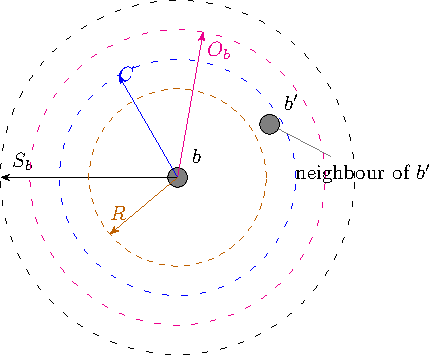
\includegraphics[width=0.8\linewidth]{figures/stableswarm}
	\caption[Agent Fields]{Agent Fields}
	\label{fig:stableswarm}
\end{figure}

\section{Related work}

As far back as 1987 swarm theory has adopted the use of field effects/potential fields to coordinate agents~\cite{REY:87} and this has continued since then in an attempt to improve the structure of a swarm, coordinate obstacle avoidance, and improve navigation~\cite{BAFVM:06,BAF:06,BFV:07,BM:09,eliot2018metric,VG:05,HC:09,SW:03,Son2017}. Improvements to the basic structure of swarms has developed through the likes of a prototype framework for self-healing swarms that was developed by Dai et al. They considered how to manage agent failure in hostile environments \cite{DHMRZ:06}. This was similar to work by Vassev and Hinchey, who modelled swarm movement using the ASSL (Autonomic System Specification Language) \cite{VH:09}. This technique was employed by NASA (US National Aeronautics and Space Administration) for use in asteroid belt exploration as part of their ANTS (Autonomous Nano Technology Swarm) project. However, this work is focused towards failure of an agent's internal systems, rather than on the removal of anomalies in a swarm distribution. This need for formation control is also discussed by Speck and Bucci with respect to the diverse applications of swarms and the need to control a swarms structure~\cite{8430773}.

In the context of swarm structure maintenance, Roach et al. focussed on the effects of sensor failure, and the impact that has on agent distribution \cite{RMT:15}. Lee and Chong identified the issue of concave edges within swarms in an attempt to create regular lattice formations \cite{GN:08}, and the main focus of their work is the dynamic restructuring of inter-agent formations. Ismail and Timmis demonstrated the use of \textit{bio-inspired} healing using \textit{granuloma formation}, a biological method for encapsulating an antigen \cite{IT:10}. They have also considered the effect failed agents can have on a swarm when traversing a terrain~\cite{TIBW:16}. 

This paper proposes an alternative approach to agent coordination that can be used to induce, among other behaviours, a void reduction effect through perimeter packing. This is an extension of the work presented by Eliot et al. \cite{eliot2019void}, Ismail and Timmis \cite{IT:10,TIBW:16}, and on the work of McLurkin and Demaine on the detection of perimeter types \cite{mclurkin2009}. However, perimeter type identification requires a communications infrastructure to allow the perimeter angle to be calculated. Communications within swarm formations limits swarm sizes and introduces performance problems \cite{fu2020formation}. The technique employed in this paper does not explicitly require the identification of the perimeter type as it would limit the size of the swarm\cite{eliot2019void,GN:08} and is therefore a reduced perimter detection algorithm to identify \textit{any} perimeter.

\section{Basic swarming model}\label{sec:basicModel}
In the Original work by Eliot et. al. the resultant vector of an agent was calculated using Equation~\ref{eq:resultantVector1a}. Where $\kc, \kr, k_d, k_o$ are weighting factors for the summed vectors associated with each interaction. i.e. $v_c$, $v_r$, $v_d$, $v_o$ for cohesion, repulsion, direction and object avoidance respectively. 

\begin{equation}\label{eq:resultantVector1a}
	v(b) = \kc v_c(b) + \kr v_r(b) + \kd v_d(b) + \ko v_o(b)
\end{equation}

Equation~\ref{eq:resultantVector1a} shows the movement vector as a linear combination of a cohesion vector $v_c$ tending to move $b$ towards its neighbours, a repulsion vector $v_r$ tending to move $b$ away from its neighbours, a direction vector  $v_d$ tending to move $b$ towards a goal, and a vector $v_o$ tending to steer it away from obstacles. $\kc, \kr, ...$ are the scalar coefficients of the the linear combination.

This paper does not consider goals or obstacles so we assume $\kd = \ko = 0$ and omit the third and fourth terms.

\subsection{Cohesion}\label{cohesion}
The cohesion component is calculated based on the proximity of neighbours. Where $n_c(b)$ is the set of neighbour agents for $b$ (Eq. \ref{eq:cohesion1}). The inclusion of an agent from a swarm ($S$) in by the agent's cohesion field ($C$).

\begin{equation}\label{eq:cohesion1}
n_c(b) = \{b' \in S~:~b' \neq b \land\magn{\vbb{b}{b'}} \leq C\}
\end{equation}

The effect of an agent being within this set is that it will generate a vector that should `encourage' agents to maintain their proximity. i.e. generate a cohesive swarm. The general weighted formula for agents to maintain their proximity is shown in Equation~\ref{eq:resultantVector1a}. Equation~\ref{eq:cohesion2} shows the technique applied to accumulating the vectors that create the cohesive effect. $\card{n_c(b)}$ denotes the cardinality of $n_c(b)$. This is the component of the overall vector calculation that has the $\kc$ quotient applied to it to allow the cohesion effect to be `balanced' with respect to other vector influences as described in ~\cite{eliot2017methods,eliot2018metric,eliot2019void}. 

\begin{equation}\label{eq:cohesion2}
v_c(b) = \frac{1}{\card{n_c(b)}} \sum_{b' \in n_c(b)}(\vbb{b}{b'})
\end{equation}

\subsection{Repulsion}\label{repulsion:neighbours}
The repulsion component of an agent's movement is calculated from interaction with its neighbours $n_r(b)$ (Eq.~\ref{eq:repulsion1a}) in a swarm ($\mathcal{S}$) that are within the agent's ($b$) repulsion field ($\rb$).

\begin{equation}\label{eq:repulsion1a}
n_r(b) = \{b' \in \mathcal{S} : b \neq b' \land \card{\vbb{b}{b'}} \leq \rb)\}
\end{equation}

The repulsion is then calculated as the average of all the vectors created by the agent ($b$) to the neighbours ($b'$) (Eg.~\ref{eq:repulsion2a}) and its proximity ($\magn{\vbb{b}{b'}} - \rb$). Where $\card{n_r(b)}$ denotes the cardinality of $n_r(b)$. This vector is then scaled to `balance' the effect with respect to other vector influences as shown is Equation~\ref{eq:resultantVector1a} where $\kc$ is applied.

\begin{equation}\label{eq:repulsion2a}
v_r(b) = \frac{1}{\card{n_r(b)}}\sum_{b' \in n_r(b)} \left(\card{\vbb{b}{b'}} - R \, \right)\widehat{\left(\vbb{b}{b'}\right)}
\end{equation}

Here, $\widehat{\vbb{b}{b'}}$ denotes $\vbb{b}{b'}$ normalized to unit length.

\section{New Inter-agent Model}
In this paper, we propose that the behaviour of an agent should be modified depending on whether or not it is on a \emph{perimeter}. Figure~\ref{fig:simplePerim2} shows a simple swarm. Perimeter agents are highlighted in \textcolor{red}{red}. Perimeter-based agents can form part of an inner boundary or an outer boundary. The swarm can also contain non-perimeter agents which are shown in black.

\begin{figure}[H]
	\begin{center}
		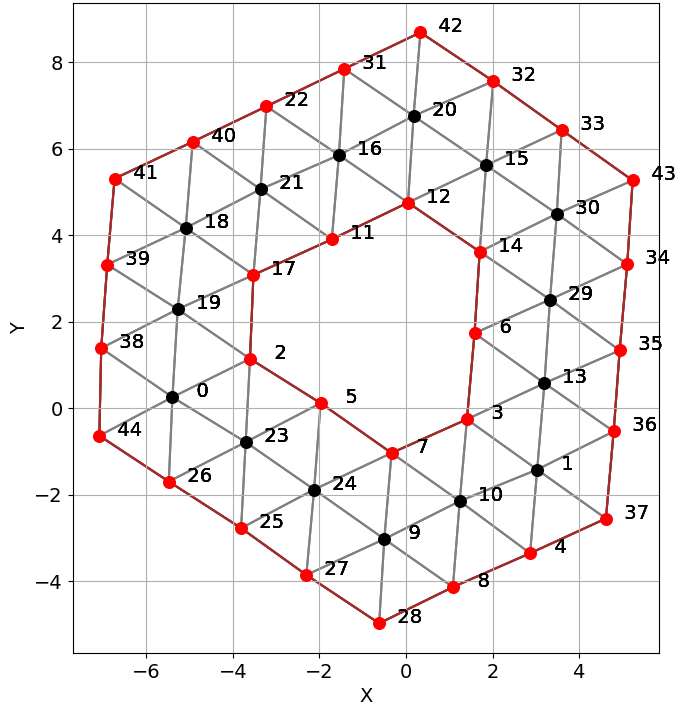
\includegraphics[width=0.8\linewidth]{figures/relationships2}
	\end{center}
	\caption{Outer and inner swarm perimeters. \label{fig:simplePerim2}}
\end{figure}

\subsection{Perimeter detection}\label{sec:perimeterDetection} 
Each agent's perimeter status is identified using a cyclic analysis of the agents (neighbours) that surround an agent~(Fig.~\ref{fig:neighbours2}). Ghrist et al. discusses a similar technique using sweep angles~\cite{ghrist2008surrounding} as does McLurkin et al~\cite{mclurkin2009}. 

When detecting a perimeter it is useful to define an ordering on an agent's cohesion neighbours. We choose to order the cohesion neighbours of an agent $b$ by their \emph{polar
angle} ($\alpha$) with respect to $b$ (Fig.~\ref{fig:neighbours2}). 

\begin{figure}[H]
	\centering
	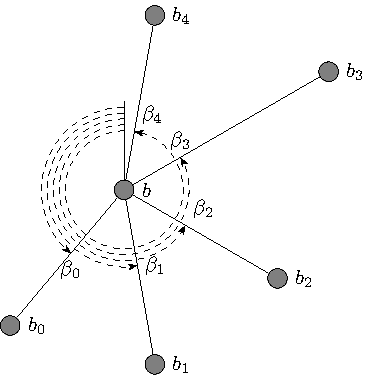
\includegraphics[width=0.8\linewidth]{figures/neighbours2}
	\caption[Agent neighbours]{Agent neighbours}
	\label{fig:neighbours2}
\end{figure}

The polar angle with respect to $b$ of $b'$,
$\pangle(b, b')$, is the counter-clockwise angle that vector $\vec{bb'} = b' - b$ makes with the positive $x$ axis shown in Figure~\ref{fig:neighbours2} as $\alpha$ and described by Equation~\ref{eq:pangle}.

\begin{equation}\label{eq:pangle}
	\pangle(b, b') = \mathsf{atan2}((\vbb{b}{b'})_y, (\vbb{b}{b'})_x)
\end{equation} 

A partial ordering of agents by polar angle with respect to a specific agent, $b$, is denoted $\leqaz{b}{}{}$, as defined in equation~\ref{angle_ordering}. 
\begin{equation}\label{angle_ordering}
	\leqaz{b}{b'}{b''} \iff \pangle(b, b') \leq \pangle(b, b'')
\end{equation}

We denote by $\angleordered{b}{b_0, b_1, .., b_{n-1}}$ a bijection from $\{0,.., n-1\} \rightarrow n_c(b)$ that is ordered by polar angle as shown in Figure~\ref{fig:neighbours3} and more formally in Equation.~\ref{angle_polar}.
\begin{equation}\label{angle_polar}
	\forall i,
j~:~0 \leq i, j, < n \cdot i \leq j \implies \leqaz{b}{b_i}{b_j}
\end{equation}

\begin{figure}[H]
	\centering
	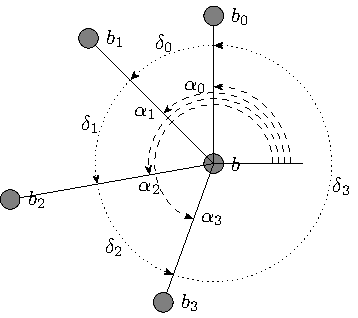
\includegraphics[width=0.8\linewidth]{figures/neighbours3}
	\caption[Agent neighbours]{Agent neighbour angles}
	\label{fig:neighbours3}
\end{figure}

An agent $b$ is on a perimeter if it satisfies any one of three conditions:
\begin{enumerate}
	\item consecutive neighbours are not within each other's cohesion field, or
	\item consecutive neighbours subtend a reflex angle (as shown in Figure~\ref{fig:neighbours3} as $\delta_3$), or
	\item the agent has too few neighbours.
\end{enumerate}
A function, $\prm(b)$, specifies these conditions formally. Let $b$ be the
agent of interest and $b'$, $b''$ any pair of consecutive neighbours of $b$ in
the angle-sorted list $\angleordered{b}{b_0, b_1, .., b_{n-1}}$, i.e. $b' =
b_i, b'' = b_{(i+1)\%n}$ for some $i \in \{0,..,n-1\}$.  Then $\prm(b)$ if any
one of the following conditions is satisfied:
\begin{enumerate}
\item $b' \notin n_c(b'')$,
\item $\delta > \pi$, where $\delta = \pangle(b, b'') - \pangle(b, b')$ (or $\delta = \pangle(b, b'') - \pangle(b, b') + 2\pi$ if the former is negative), or
\item $\card{n_c(b)} < 3$.
\end{enumerate}

\subsection{$\rb$, $\kr$ and $\kc$}\label{sec:rbkrkc} 
This section discusses the application of the new $\rb$, $\kr$ and $\kc$ two dimensional ($2\times2$) arrays structured as shown below:

\[
  \kbordermatrix{
                   & \text{False} & \text{True} \\
    \text{False}   & i\rightarrow i   & i\rightarrow p  \\
    \text{True}    & p\rightarrow i   & p\rightarrow p
  }
\]

Where \emph{i} represents an internal agent and \emph{p} is a perimeter agent. If we consider Figure~\ref{fig:simplePerim2} then agents $18\rightarrow 21$ would be internal to internal ($i-i$), $18\rightarrow 39$ would be internal to perimeter ($i-p$), $39\rightarrow 19$ would be perimeter to internal ($p-i$) and $41\rightarrow 40$ would be perimeter to perimeter ($p-p$).

The new model requires each agent to modify their inter-agent repulsion and cohesion vectors based upon their perimeter status and each neighbour's perimeter status. The basic perimeter control technique is shown in Equation~\ref{eq:newModel2} where the cohesion and repulsion arrays ($\kc$, $\kr$, $\rb$) are integrated into $v_c(b)$ and $v_r(b)$.

\begin{equation}\label{eq:newModel2}
v(b) = v_c(b) + v_r(b)
\end{equation}\\

\subsubsection{Cohesion vector}~\\
Cohesion neighbours are identified as  described in Equation~\ref{eq:cohesion1}. The cohesion influence is then calculated as shown in Equation~\ref{eq:coh2}.
\begin{equation}\label{eq:coh2}
	v_c(b) = \frac{1}{|n_c(b)|} \sum_{b' \in n_c(b)} \kc[p_b, p_{b'}] (b' - b)
\end{equation}
where $|n_c(b)|$ denotes the cardinality of $n_c(b)$, $p_b = \prm(b)$, $p_{b'} 
= \prm(b')$, and 
$\kc$ is a 2x2 boolean-indexed array of constants that determine the weight
of a component of the cohesion vector according to
whether the interaction between $b,b'$ is between non-perimeter agents,
non-perimeter--perimeter, perimeter--non-perimeter, or perimeter--perimeter
agents.

\subsubsection{Repulsion vector}~\\
~\\
The set of repellers of $b$ are defined as Equation~\ref{eq:rep1}.
\small
\begin{equation}\label{eq:rep1}
	n_r(b) = \{b' \in \mathcal{S} : b \neq b' \wedge \vbb{b}{b'} \leq \rb[p_b,p_{b'}]\}
\end{equation}
\normalsize
where $p_b = \prm(b)$, $p_{b'} = \prm(b')$, and $\rb$ is a 2x2 boolean-indexed
array of constants that determine the radius of the \emph{repulsion field} for agents in the swarm, according to whether the interaction between $b,b'$ is between non-perimeter agents, non-perimeter--perimeter,
perimeter--non-perimeter, or perimeter--perimeter agents.\\

Now $v_r(b)$ is defined by Equation~\ref{eq:rep2}
\small
\begin{equation}\label{eq:rep2}
	v_r(b) = \frac{1}{\magn{n_r(b)}}\sum_{b' \in n_r(b)} \kr[p_b,p_{b'}] \left(1 - \frac{\rb[p_b,p_{b'}]}{\vbb{b}{b'}} \, \right) (\vbb{b}{b'})
\end{equation}
\normalsize
where $p_b = \prm(b)$, $p_{b'} = \prm(b')$, and $\kr$ is a 2x2 boolean-indexed
array of constants that determine the weight of a component of the repulsion
vector according to whether the interaction between $b,b'$ is between
non-perimeter agents, non-perimeter--perimeter, perimeter--non-perimeter, or
perimeter--perimeter agents.

\subsection{Gap-filling}

In addition to cohesion and repulsion vectors, a \emph{gap-filling} vector can
also be used to contribute to agent behaviour. Gap-filling vectors have proven
useful in quickly reducing internal voids and in controlling the shape of the
external perimeter.

A gap-filling vector for $b$ contributes a motion of $b$ towards the midpoint
of a gap identified in the perimeter test for $b$.

Let $\angleordered{b}{b_0, b_1, .., b_{n-1}}$ be the cohesion neighbours of $b$
in polar angle order, and let $b' = b_i$  and $b'' = b_{(i+1)\%n}$ be the first
pair of consecutive neighbours that satisfy either condition (1) or condition
(2) of the perimeter function $\prm()$, then the gap-filling vector, $v_g(b)$,
for agent $b$ is defined in Equation~\ref{eq:gap1}.
\small
\begin{equation}\label{eq:gap1}
v_g(b) = \kg \left (\frac{b' + b''}{2} - b \right) = \kg \frac{\vbb{b}{b'} + \vbb{b}{b''}}{2} 
\end{equation}
\normalsize
If there is no such pair of consecutive neighbours then $v_g(b) = 0$.

$\kg$ is a weighting for the gap-filling vector allowing the combination of it
with the other motion vectors (cohesion, repulsion, ...) to be ``tuned''.

A stricter alternative to this is to choose the first consecutive neighbour
pair $b',b''$ that satisfy condition (1), ignoring condition (2).  This would then exclude any reflex angles that create a `gap'.Again, $v_g(b)$ is defined by eq (\ref{eq:gap1}) if such a pair exists, or 0 otherwise.

\subsection{Resultant vector}
The resultant vector is simply the sum of the cohesion, repulsion and
gap-filling vectors as shown in Equation~\ref{eq:res} and a resulant swarm segment is shown in Figure~\ref{fig:swarmExample}
\begin{equation}\label{eq:res}
	v(b) = v_c(b) + v_r(b) + v_g(b) 
\end{equation}

\begin{figure}[H]
	\begin{center}
		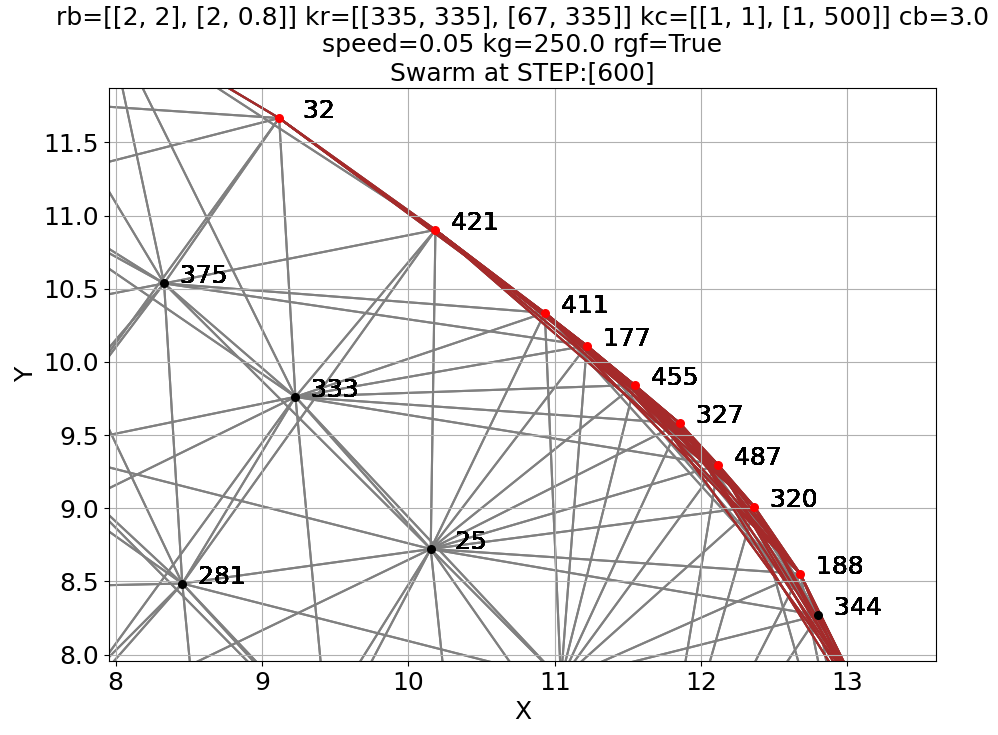
\includegraphics[width=8cm]{figures/perimeterCompress}
	\end{center}
	\caption{Swarm Example.\label{fig:swarmExample}}
\end{figure}

\subsection{Relationship-based swarm effects}

The introduction of the arrays allows for specific relationships to effect the movement of agents. Using uniform arrays results a simple cohesion/repulsion based swarm with all agents exhibiting the same properties similar to the original model discussed in \S~\ref{sec:basicModel}. However, modifying the arrays for specific relationships can induce emergent behaviours such as perimeter packing as discussed in \S~\ref{sec:perimCompress}.

\subsubsection{Cohesion model}~\\
When using Equation~\ref{eq:coh2} one array is used, $k_c$. This array is used to scale the cohesion vector generated between an agent pair which is proportional to their distance apart, which will be within $C$ as shown in Equation~\ref{eq:repulsion1a}. Consider the array shown in Equation~\ref{eq:kcexample1}.

\begin{equation}\label{eq:kcexample1}
	\kc = 
	\begin{bmatrix}
	1 & 1\\
	1 & 500
	\end{bmatrix}
\end{equation}

For a given agent pair their perimeter status will be calculated and applied to the arrays. If both agents are perimeter based then the value selected would be $k_c[P_b,P_{b'}]\Rightarrow 500$. If the agent pair were perimeter $\rightarrow$ non-perimeter then the value selected would be $k_c[P_b,P_{b'}]\Rightarrow 1$. This configuration would cause inter-perimeter agents to tend to move towards each other more strongly than any other relationship.

\subsubsection{Repulsion model}~\\
When using Equation~\ref{eq:rep2} two arrays are used $\kr$ and $\rb$. $\kr$ is used to scale the resultant repulsion vector that is generated. $\rb$ is the radius of the repulsion field and is used to generate the proportion of the repulsion vector that is applied. Therefore consider the following two arrays (Eqs~\ref{eq:rexample1}~and~\ref{eq:krexample1}):

\begin{equation}\label{eq:rexample1}
	\rb = 
	\begin{bmatrix}
	2 & 2\\
	2 & 0.8
	\end{bmatrix}
\end{equation}

\begin{equation}\label{eq:krexample1}
	\kr = 
	\begin{bmatrix}
	335 & 335\\
	67 & 335
	\end{bmatrix}
\end{equation}

For a given agent pair their perimeter status will be calculated and applied to the arrays. If both agents are perimeter based then the values selected would be $\rb[P_b,P_{b'}]\Rightarrow 0.8$ and $\kr[P_b,P_{b'}]\Rightarrow 335$. If the agent pair were perimeter $\rightarrow$ non-perimeter then the values selected would be $\rb[P_b,P_{b'}]\Rightarrow 2$ and $\kr[P_b,P_{b'}]\Rightarrow 67$.\\

\section{Experimental results\label{sec:ExperimentalResults}}
The new modelling method allows for a highly configurable swarm. Each configuration will have an impact on the a swarm's structural changes. This can be analysed in several different ways. This includes the magnitude of the interactions between agents and the distances between the agents. The experimental results show the effects on the swarm in terms of inter-agent distances, magnitude metric~\cite{eliot2018metric}, and the effect on the perimeter. The section will cover three experiments. Only one experiment will be covered under baseline 1 as a an expanded perimeter will only form from an initial deployment that involves a compressed swarm or is confined in some manner.

\subsection{Distance metric}
The distance metric is used by many researchers as a method of examining the structure of a swarm~\cite{BAFVM:06,BAF:06,elamvazhuthi2015optimal,VG:05,SW:03}. However, due to the new model allowing the field effects and magnitudes to be varied the distance metric will need to be adapted to analyse the agents involved in specific relationships rather than globally, therefore $S$ will be sub-divided into the three relationship categories of $S_i$, $S_p$, $S_{o}$. Where $S_i$ are the internal-internal relationships, $S_p$ are the perimeter-perimeter relationships and $S_{o}$ are all the internal-perimeter or perimeter-internal relationships. 
The distance metric is based upon the mean of a set of agents distances from its neighbours and the standard deviation between those agent sets. The mean is calculated as shown in equation~\ref{eq:SwarmStabilityDistance2} where $\mu_d(S)$ is the mean. The standard deviation is calculated as shown in equation~\ref{eq:SwarmStabilityDistance3} where $\sigma_d(S)$ is the standard deviation. The mean distance value can be compared to the repulsion field to identify if a swarm is optimally distributed in that the mean value should be as close to the repulsion filed as possible. The standard deviation identifies the overall differences in the distances which can be caused by the swarm agents oscillating. A standard deviation of $\sigma_d(S) = 0$ would indicate that all the agents are equally spaced.
\small
\begin{equation}
\label{eq:SwarmStabilityDistance2}
\mu_d(S) = \frac{\mathlarger{\sum_{b \in S}}~\mathlarger{\sum_{b' \in nbr(b)}}\card{\vbb{b}{b'}}}{\mathlarger{\sum_{b \in S}\card{nbr(b)}}}
\end{equation}
\normalsize
\small
\begin{equation}
\label{eq:SwarmStabilityDistance3}
\sigma_d(S) = \sqrt{\frac{\mathlarger{\sum_{b \in S}}~\mathlarger{\sum_{b' \in nbr(b)}}\Big(\card{\vbb{b}{b'}} - \mu_d(S)\Big)^2}{\mathlarger{\sum_{b \in S}\card{nbr(b)}}}}
\end{equation}
\normalsize

Therefore the distance metric for the distribution of a set of agents is both $\mu_d(S)$ and $\sigma_d(S)$. This can be written informally as:

\small
\begin{equation}
\label{eq:SwarmPotentialMagnitude}
\psi_d(S) = \mu_d(S)\pm \sigma_d(S)
\end{equation}
\normalsize

An example is shown in Figure~\ref{fig:tightPerimDistance}.

\subsection{Magnitude metric}
The magnitude metric as defined by Eliot et al.~\cite{eliot2018metric} is based upon the relationship between agents and as such is independent of the resultant structure in terms of distances. i.e. agents can be different distances from each other but have the same relationship magnitude.
The metric is based upon the mean of a set of agent relationships and the standard deviation between those relationships. The mean is calculated as shown in equation~\ref{eq:SwarmStabilityMetricT3} where $\mu_p(S)$ is the mean. The standard deviation is calculated as shown in equation~\ref{eq:SwarmStabilityQuotientT} where $\sigma_p(S)$ is the standard deviation. Due to the metric being based on inter-agent relationships the swarm can be analysed as a whole.

\small
\begin{equation}
\label{eq:SwarmStabilityMetricT3}
\mu_p(S) = \frac{\mathlarger{\sum_{b \in S} P(b)}}{\mathlarger{\sum_{b \in S}}\card{nbr(b)} + \mathlarger{\sum_{b \in S}}\card{n_r(b)}}
\end{equation}
\normalsize
\small
\begin{equation}
\label{eq:SwarmStabilityQuotientT}
\sigma_p(S) = \sqrt{\frac{\mathlarger{\sum_{b \in S}}\Big(P(b)-\mu_p(S)\Big)^2}{\mathlarger{\sum_{b \in S}}\card{nbr(b)} + \mathlarger{\sum_{b \in S}}\card{n_r(b)}}}
\end{equation}
\normalsize

The metric for the internal movement is the mean and standard deviation of the swarm's internal \emph{cohesion/repulsion}. The pair $\mu_p(S)$, $\sigma_p(S)$ may therefore be written informally as: 

\small
\begin{equation}
\label{eq:SwarmMagnitudeMatric}
\psi_p(S) = \mu_p(S)\pm \sigma_p(S)
\end{equation}
\normalsize

\subsection{Baseline Settings}
For all the experiments the parameters used to create the basic swarming effect are shown in Table~\ref{tab:swarmingEffect}. Where $C$ is the cohesion field, $\kc$ is the cohesion weighting, $\rb$ is the repulsion field, $\kr$ is the repulsion weighting and $\kg$ is the weighting applied in the gap reduction algorithm discussed in~\cite{eliot2019void}. 

\begin{table}[H]
	\centering
	\tiny
	\begin{tabular}{|c|r|}
		\hline
		\rowcolor[HTML]{000000} 
		{\color[HTML]{FFFFFF} Swarming Variable} & {\color[HTML]{FFFFFF} Value} \\ \hline
		$C$ & \texttt{3.0} \\ \hline
		$k_c$ & \texttt{[[1.0,1.0][1.0,1.0]]}  \\ \hline
		$R$ & \texttt{[[2.0,2.0][2.0,2.0]]} \\ \hline
		$k_r$ & \texttt{[[335,335][335,335]]} \\ \hline
		$k_g$ & \texttt{0.0} \\ \hline
	\end{tabular}
	\caption{Swarming effect parameters}
	\label{tab:swarmingEffect}
\end{table}

\subsection{Baseline 1}
The first swarm consists of 500 agents which are distributed with a void at the centre. These initial parameters create a hexagonal-based distribution of agents that stabilise as shown in Figure~\ref{fig:baselineSwarm}. 

\begin{figure}[H]
	\begin{center}
		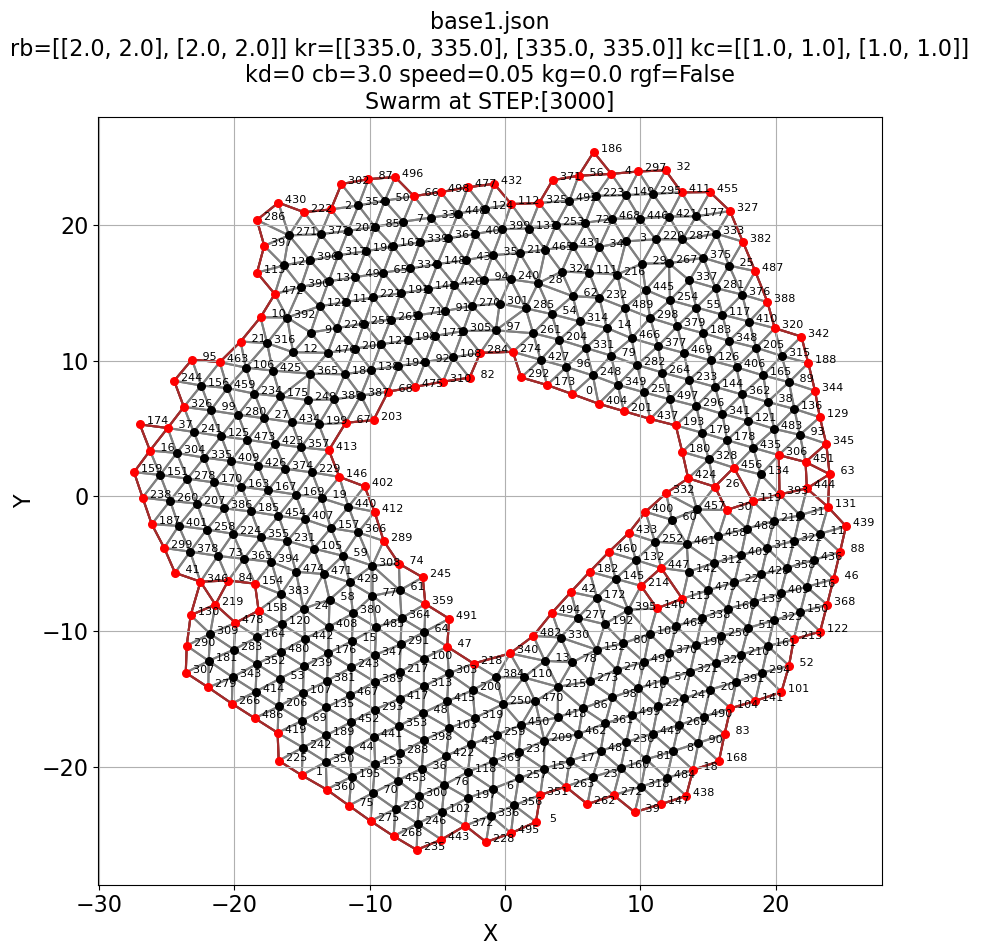
\includegraphics[width=1.0\linewidth]{figures/baseline}
	\end{center}
	\caption{Baseline swarm. \label{fig:baselineSwarm}}
\end{figure}

When the simulation is ran with no relationship differences i.e. all array values are equal, the changes are identified using a magnitude-based metric~\cite{eliot2018metric}. The resultant magnitudes generated are shown in figure~\ref{fig:baselineMagnitude}. The swarm is also analysed based on the inter-agent distances as shown in figure~\ref{fig:baselineDistance}. The distance graph shows the different agent relationships types split into $S_{i}$, $S_{p}$ and $S_{o}$ to allow a comparison with the new model. This state is used as the baseline for the experiments to measure the effects of changing the new arrays. The baseline configuration is equivalent to the conventional swarming algorithms using single value potential fields.

The magnitude graph (Fig.~\ref{fig:baselineMagnitude}) shows that the swarms is relatively stable in that the overall magnitude is around 8 and there is a standard deviation of around 5 which means the swarms internal magnitude ranges between 3 and just over 12.

\begin{figure}[H]
	\begin{center}
		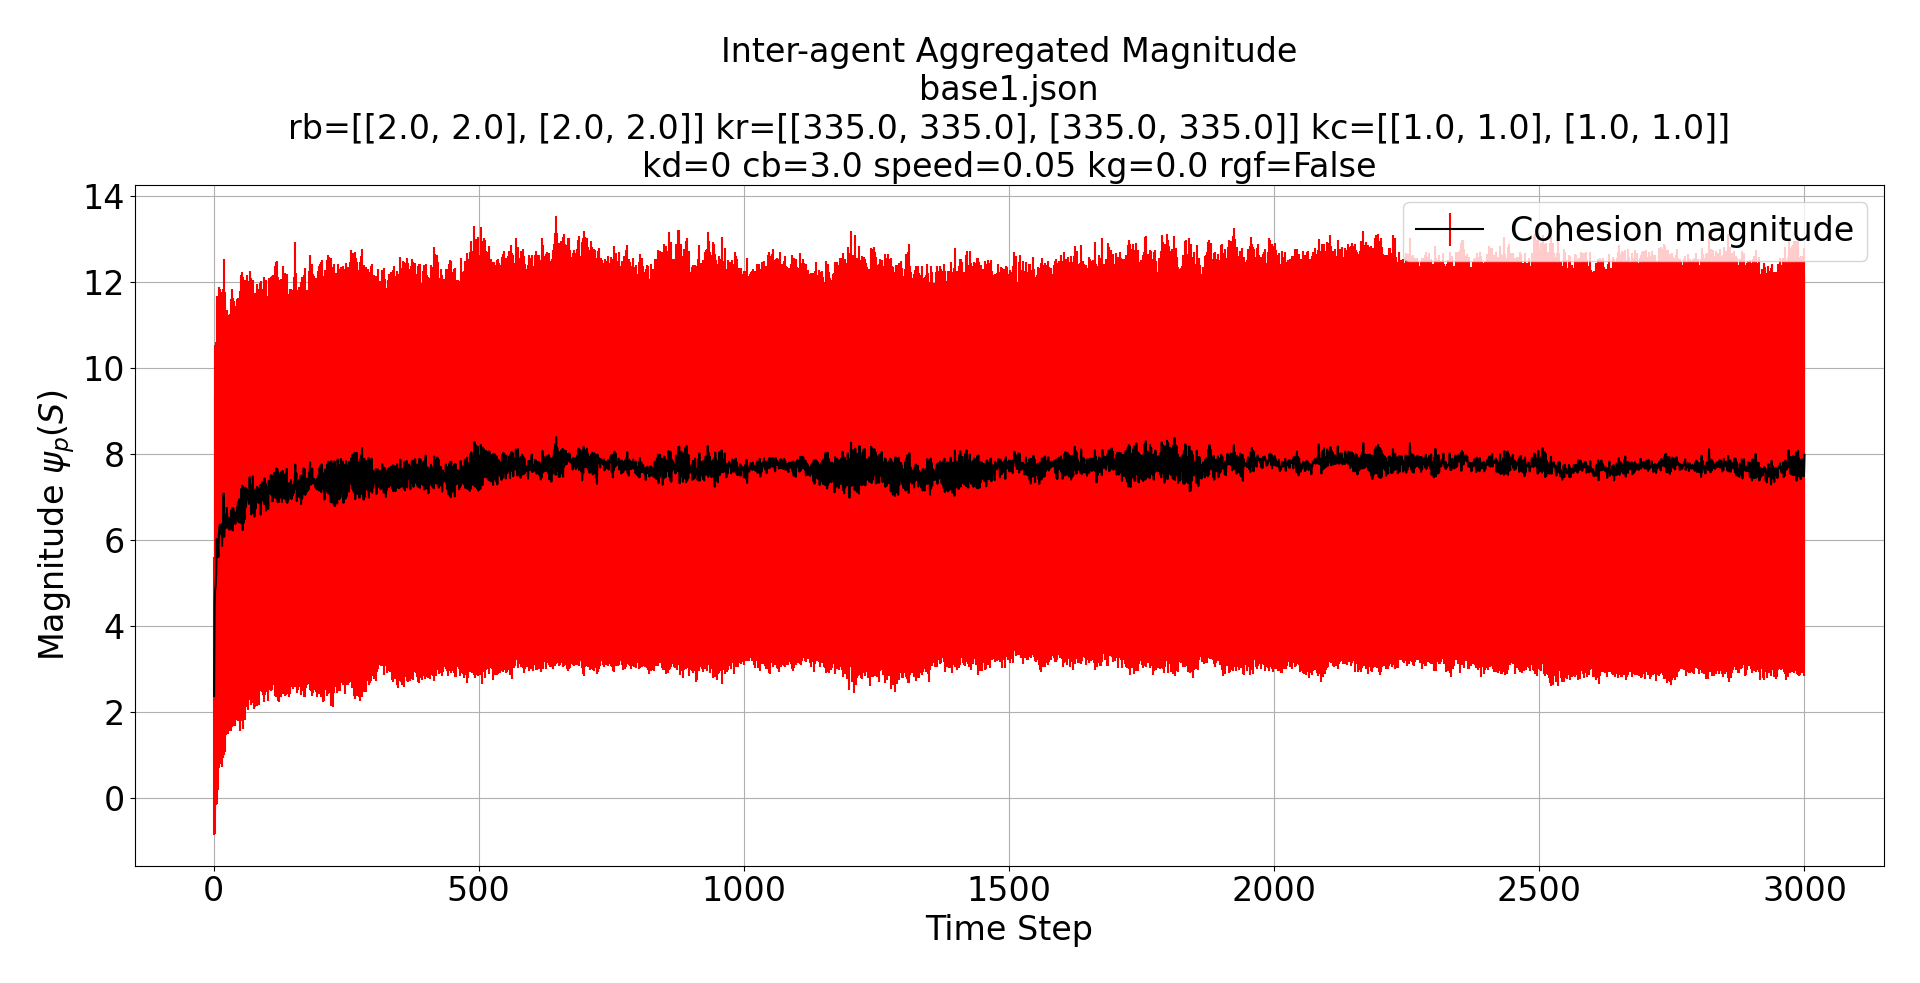
\includegraphics[width=1.0\linewidth]{figures/baselineMagnitude}
	\end{center}
	\caption{Baseline swarm (Magnitude). \label{fig:baselineMagnitude}}
\end{figure}

The distance graph shows that perimeter-perimeter agents and the settle to a similar average distance of around 2.07 units and the internal agents settle to around 2.04 units. Given that the repulsion field is set to 2 units the swarm looks very stable and is able to form a lattice based structure that changes very little and has a small amount of jitter. Jitter is the slight variation in position that agents exhibit as they move to more optimum positions.

\begin{figure}[H]
	\begin{center}
		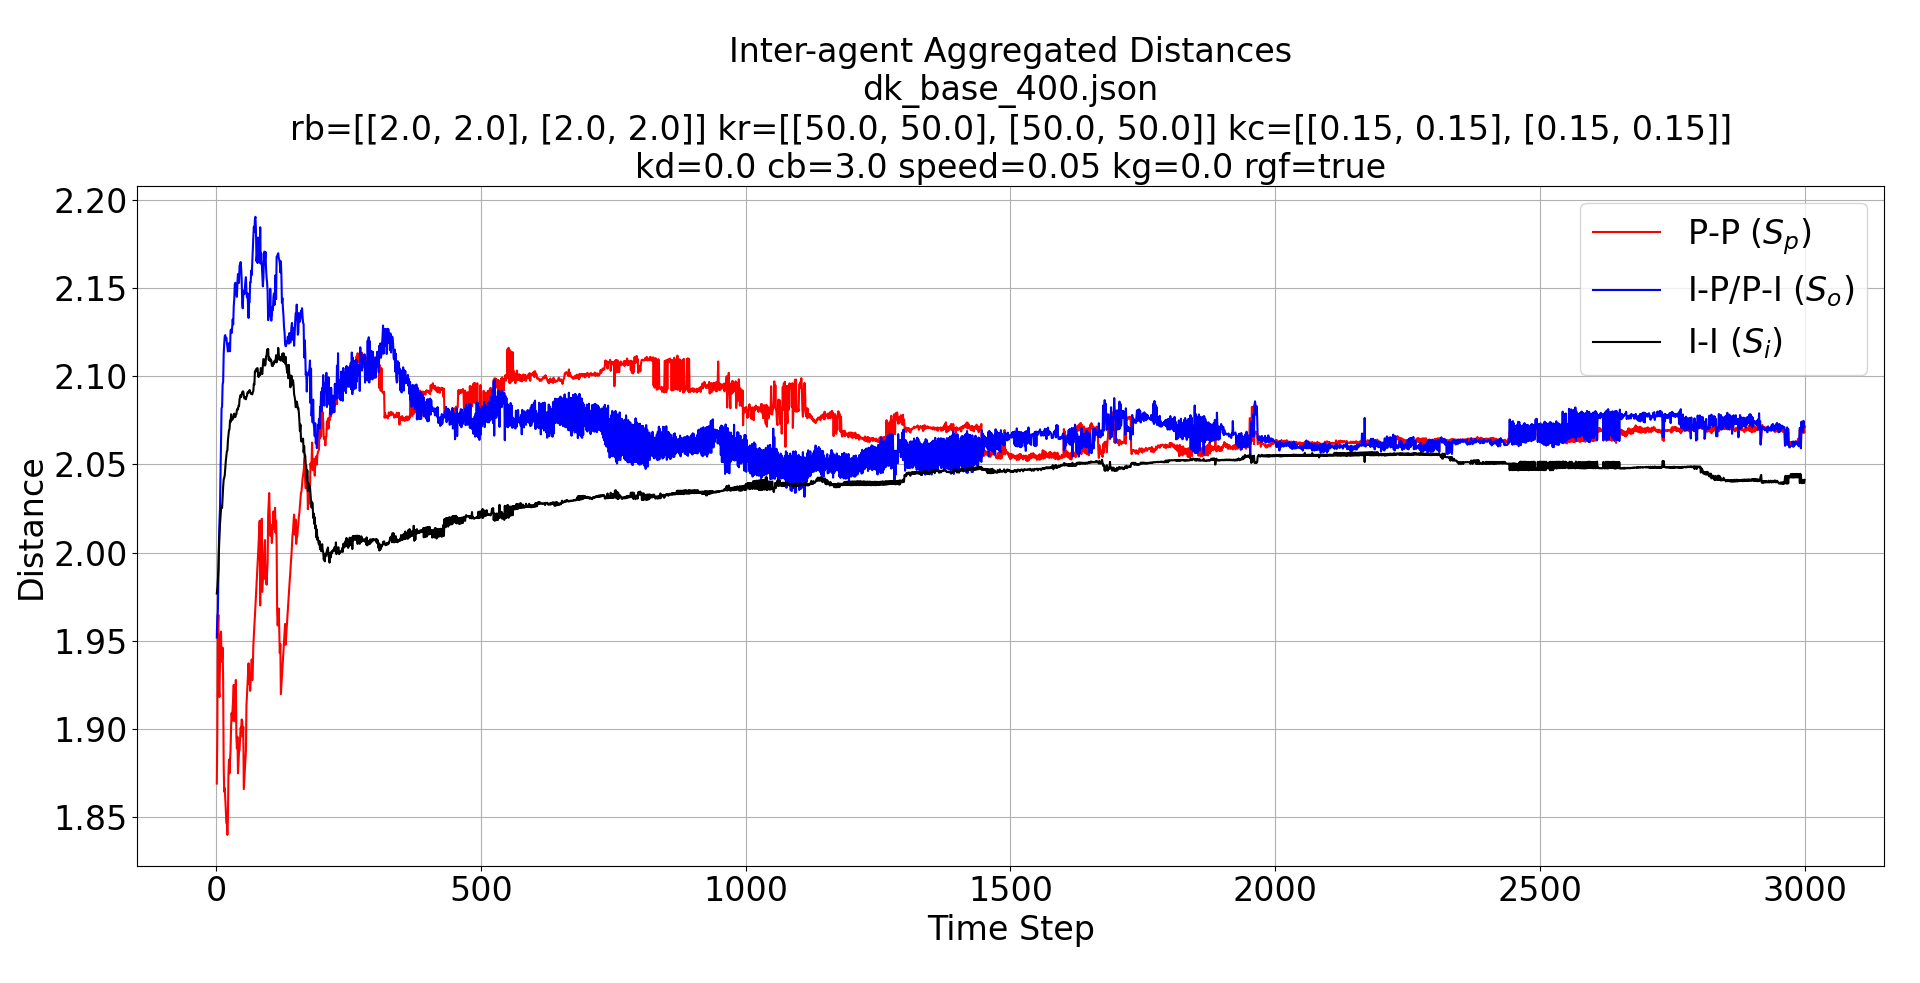
\includegraphics[width=1.0\linewidth]{figures/baselineDistance}
	\end{center}
	\caption{Baseline swarm (Distance). \label{fig:baselineDistance}}
\end{figure}

\subsubsection{Perimeter Packing and Void Removal}\label{sec:perimCompress}

The first experiment with the new model is to create a swarm that has a densely packed perimeter and exhibits a self-healing behaviour. This is achieved by modify the perimeter\textrightarrow perimeter agents relationship and the perimeter\textrightarrow non-perimeter/non-perimeter\textrightarrow perimeter relationship. The perimeter\textrightarrow perimeter agent repulsion field is reduced (Eq.~\ref{eq:rbexp1}) and the cohesion weighting is increased (Eq.~\ref{eq:kcexp1}), next the repulsion weighting of the  perimeter\textrightarrow non-perimeter/non-perimeter\textrightarrow perimeter agents is reduced to allow the perimeter agents to pull closer together without the next layer of agents reducing the effect (Eq.~\ref{eq:krexp1}). The effect here is that the perimeter agents are able to have more internal neighbours before the aggregate repulsion prevents them moving into closer proximity of each other as shown in figure~\ref{fig:tightPerim2}. As well as those changes a gap reduction effect is added ($\kg=250$). This effect includes closing the reflex angle ($\rgf=\mathsf{True}$) to smooth the perimeter and cause a  compression on a perimeter. Using a high $\kg$ value creates a circular shaped swarm and stabilises the structure (Fig.~\ref{fig:tightPerim}).

\begin{equation}\label{eq:rbexp1}
\rb = 
\begin{bmatrix}
2.0 & 2.0\\
2.0 & 1.0
\end{bmatrix}
\end{equation}

\begin{equation}\label{eq:krexp1}
\kr = 
\begin{bmatrix}
335 & 5.0\\
5.0 & 335
\end{bmatrix}
\end{equation}

\begin{equation}\label{eq:kcexp1}
\kc = 
\begin{bmatrix}
1.0 & 1.0\\
1.0 & 10.0
\end{bmatrix}
\end{equation}

\begin{figure}[H]
	\begin{center}
		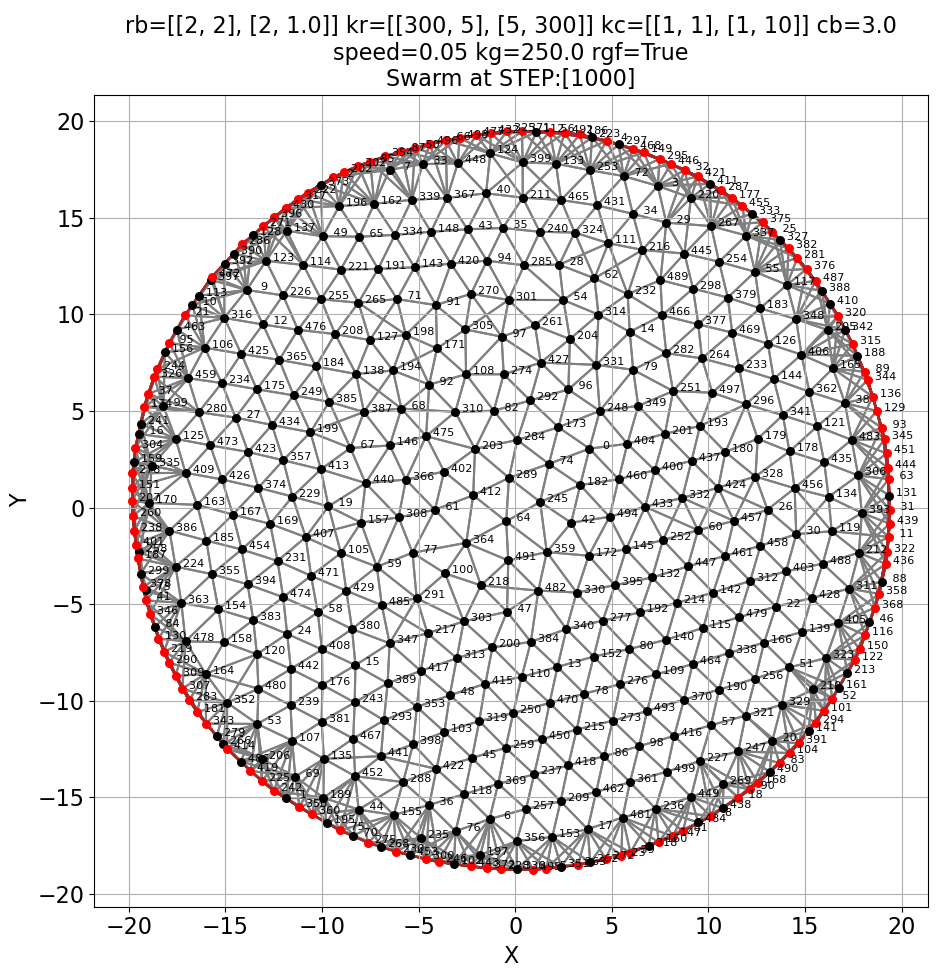
\includegraphics[width=1.0\linewidth]{figures/tightPerim}
	\end{center}
	\caption{Packed Perimeter. \label{fig:tightPerim}}
\end{figure}

\begin{figure}[H]
	\begin{center}
		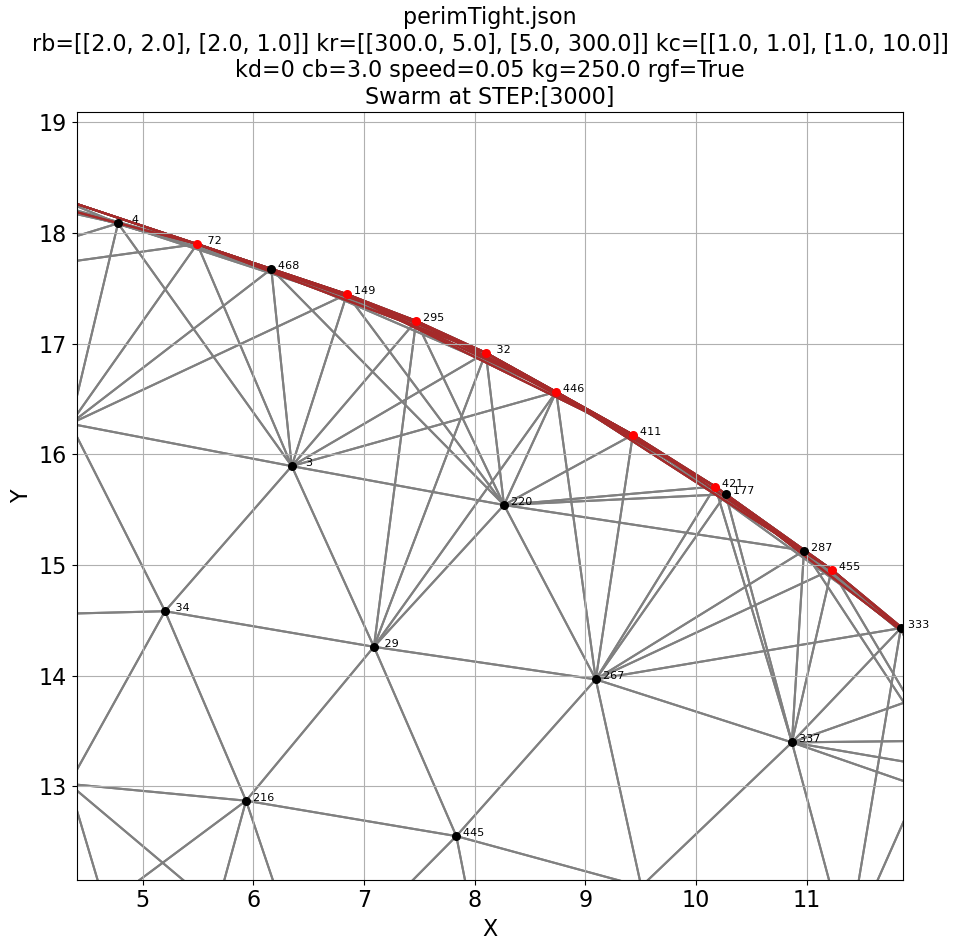
\includegraphics[width=1.0\linewidth]{figures/tightPerim2}
	\end{center}
	\caption{Packed Perimeter. \label{fig:tightPerim2}}
\end{figure}

The effect of the parameters effects the swarm by causing a change in the distribution of the agents compared to baseline 1. Figure~\ref{fig:tightPerimDistance} shows that the perimeter agents ($S_{p}$) are now closer together but also shows that the distribution of the p\textrightarrow i and i\textrightarrow p agents ($S_{i}$, $S_{o}$) are now of a similar distance apart which allows the internal agents to form a regular hexagonal lattice.

\begin{figure}[H]
	\begin{center}
		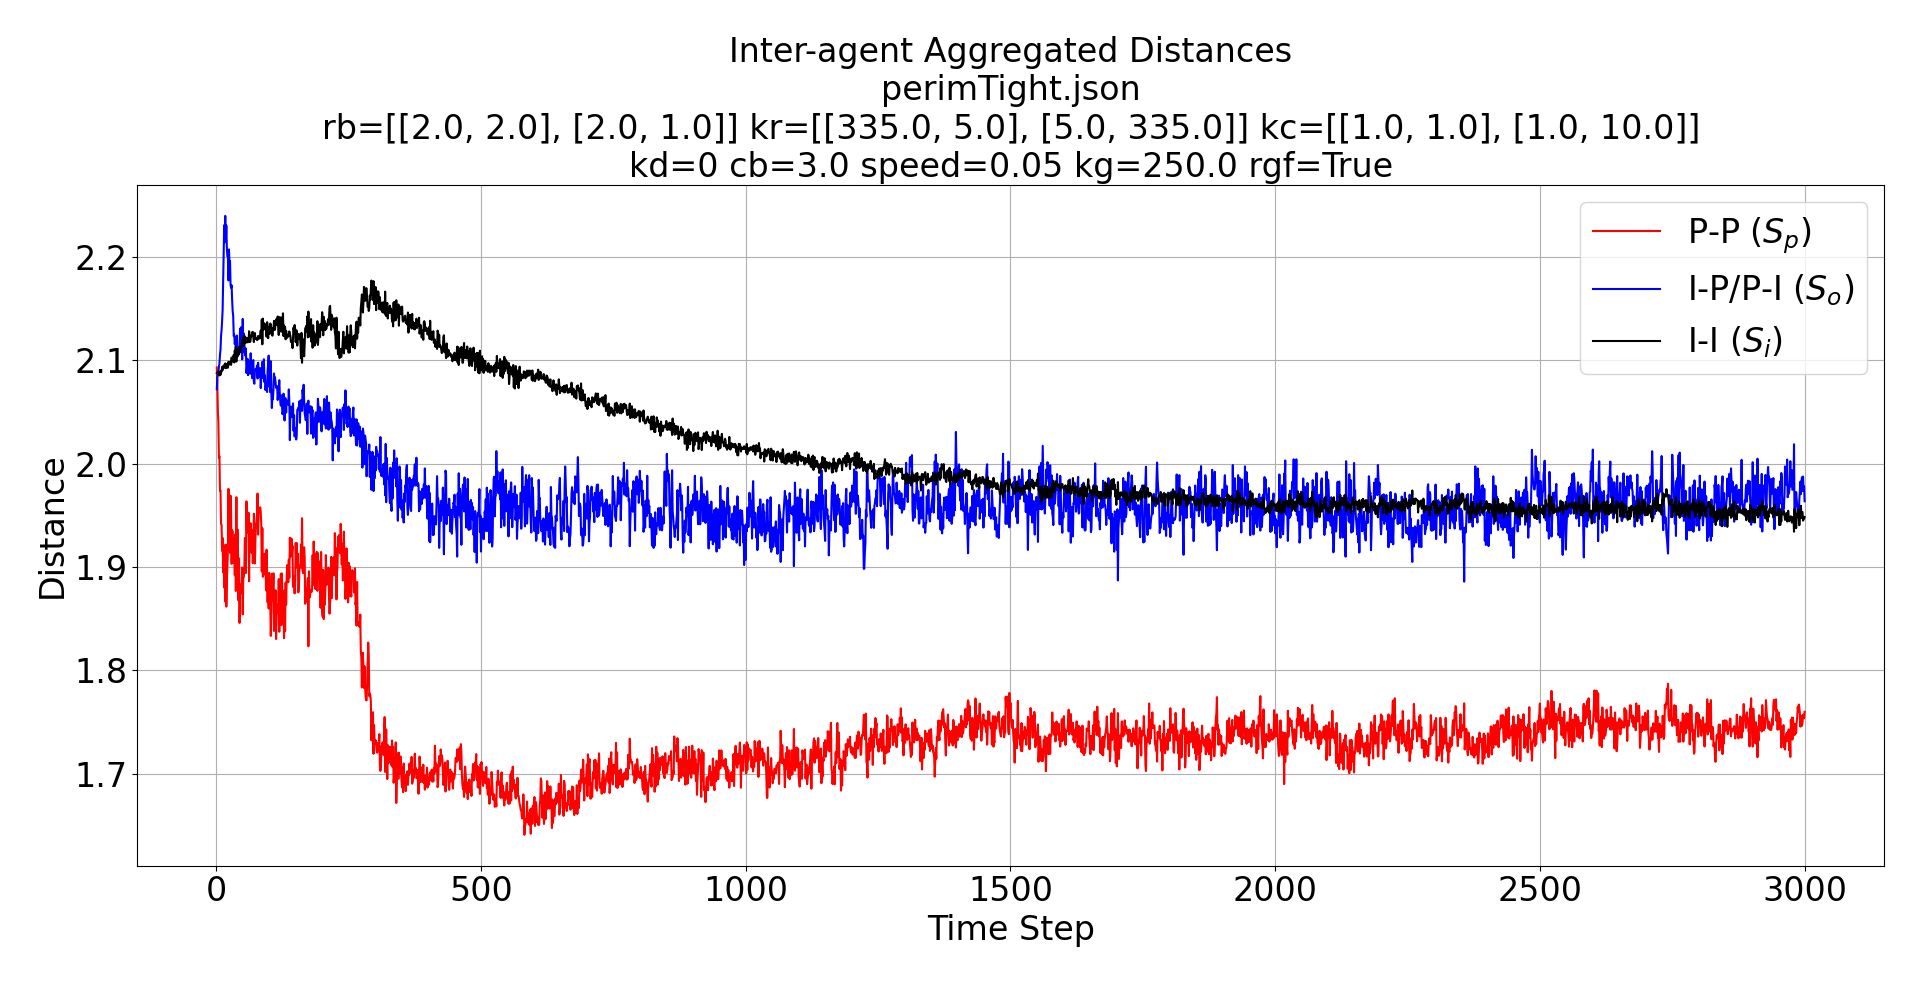
\includegraphics[width=1.0\linewidth]{figures/tightPerimDistance}
	\end{center}
	\caption{Packed Perimeter (Distance). \label{fig:tightPerimDistance}}
\end{figure}

In terms of the magnitude relationships, shown in graph~\ref{fig:tightPerimMagnitude}. The agents are effected by the compression of the perimeter. This is shown by the increased average magnitude within the swarm. The metric also shows that the packing and compression on the perimeter cause more of a disturbance within the sarm which is shown by the increased standard deviation from the mean magnitude.

\begin{figure}[H]
	\begin{center}
		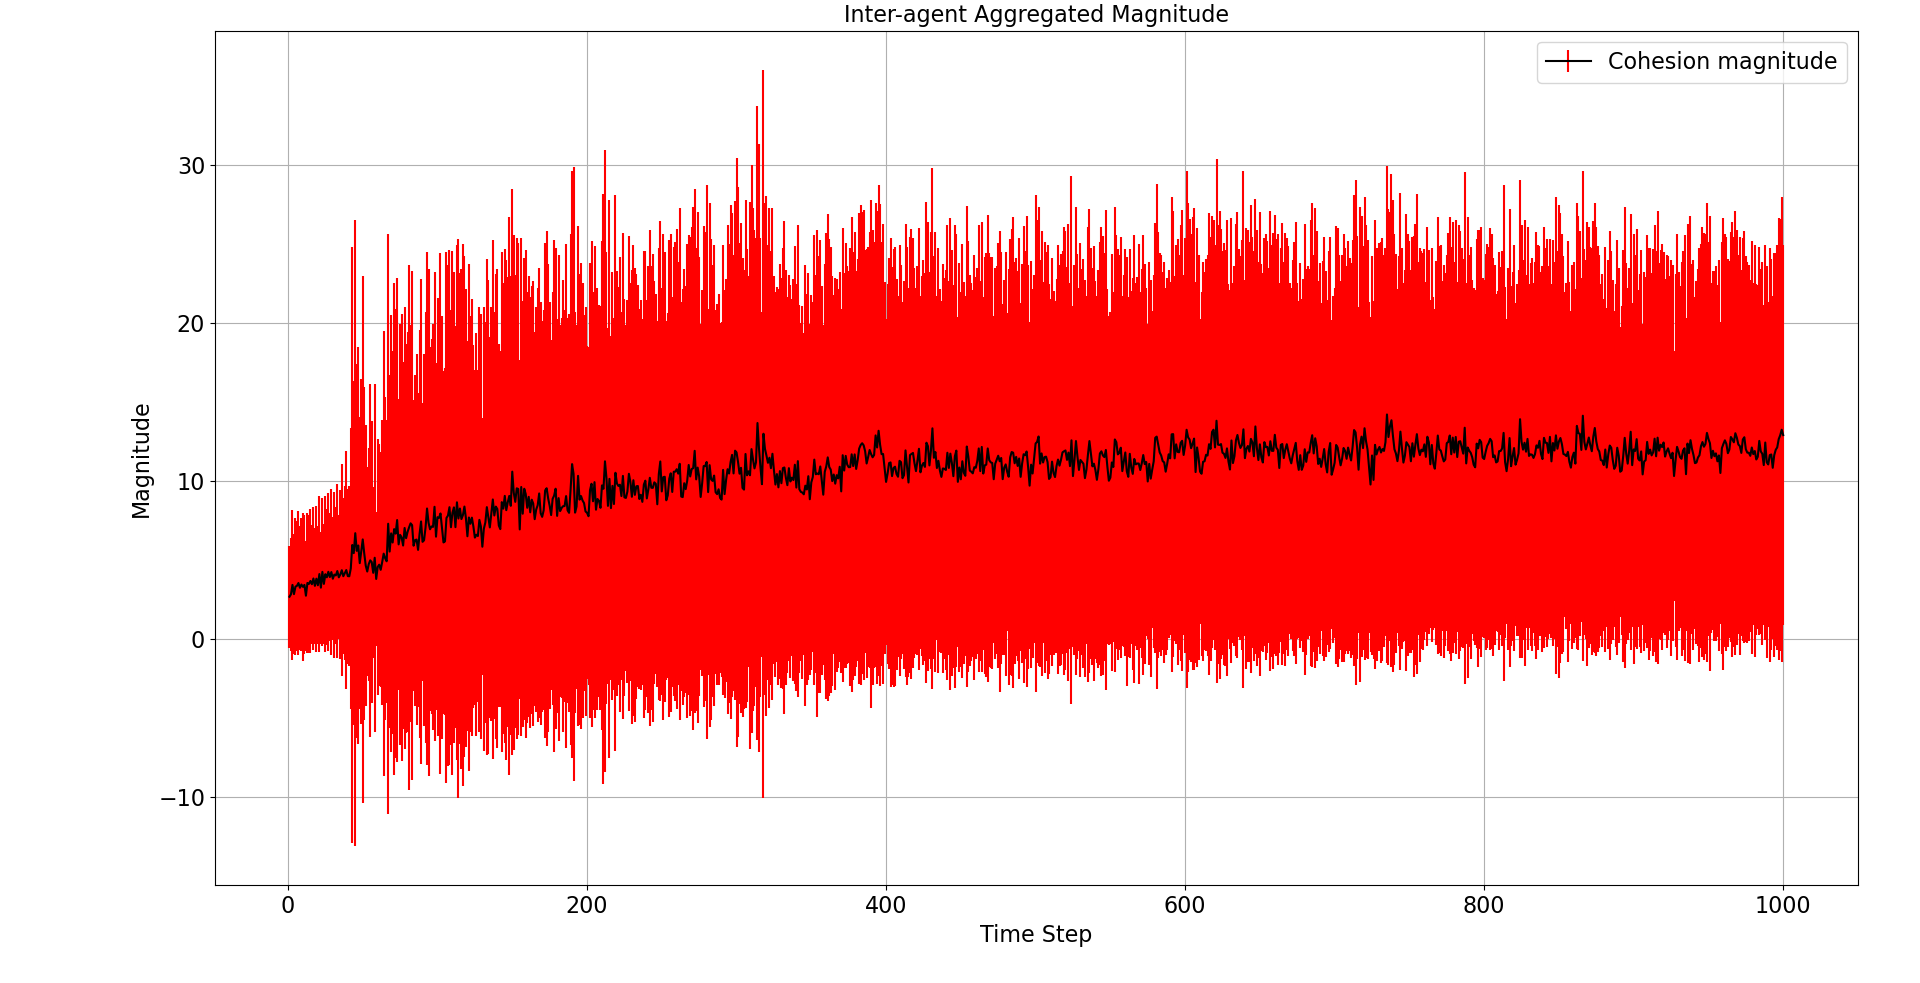
\includegraphics[width=1.0\linewidth]{figures/tightPerimMagnitude}
	\end{center}
	\caption{Packed Perimeter (Magnitude). \label{fig:tightPerimMagnitude}}
\end{figure}

\subsection{Baseline 2}
The second swarm consists of 500 agents which are distributed within a small area to create a compressed swarm as shown in Figure~\ref{fig:baseline2}. These initial parameters create a hexagonal-based distribution of agents that stabilise as shown in Figure~\ref{fig:baseline2-2}. This configuration is equivalent to the conventional swarming algorithms using single value potential fields. 

\begin{figure}[H]
	\begin{center}
		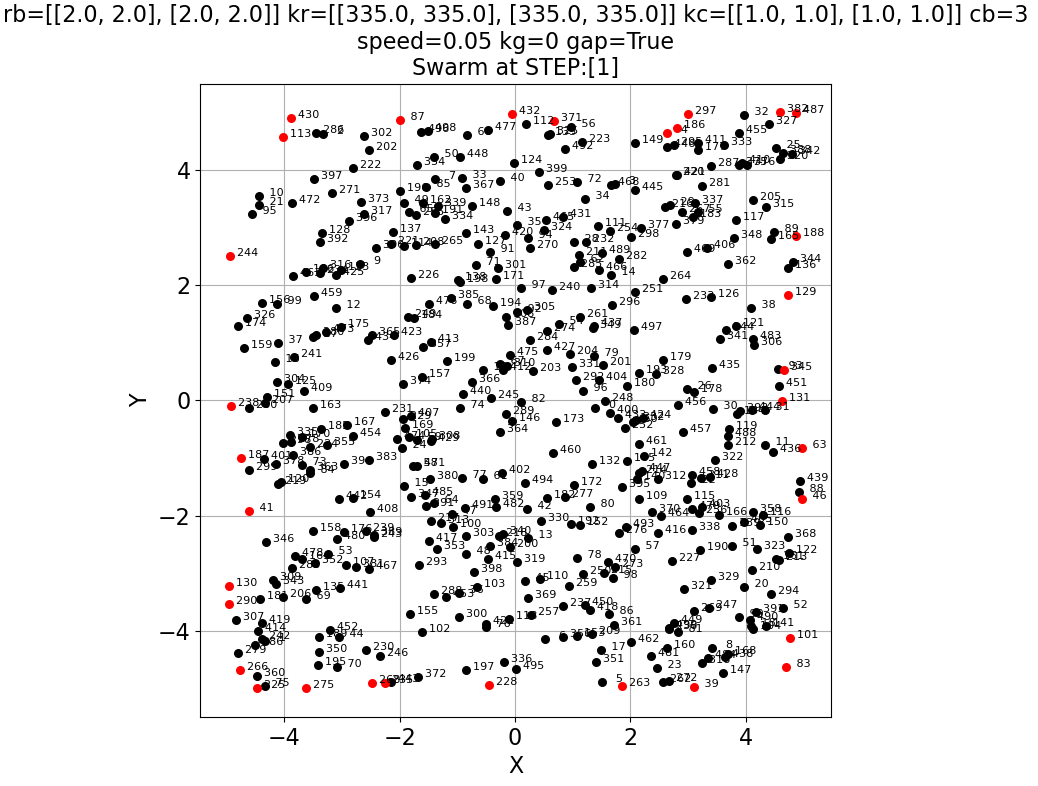
\includegraphics[width=1.0\linewidth]{figures/baseline2-1}
	\end{center}
	\caption{Baseline 2 start. \label{fig:baseline2}}
\end{figure}

\begin{figure}[H]
	\begin{center}
		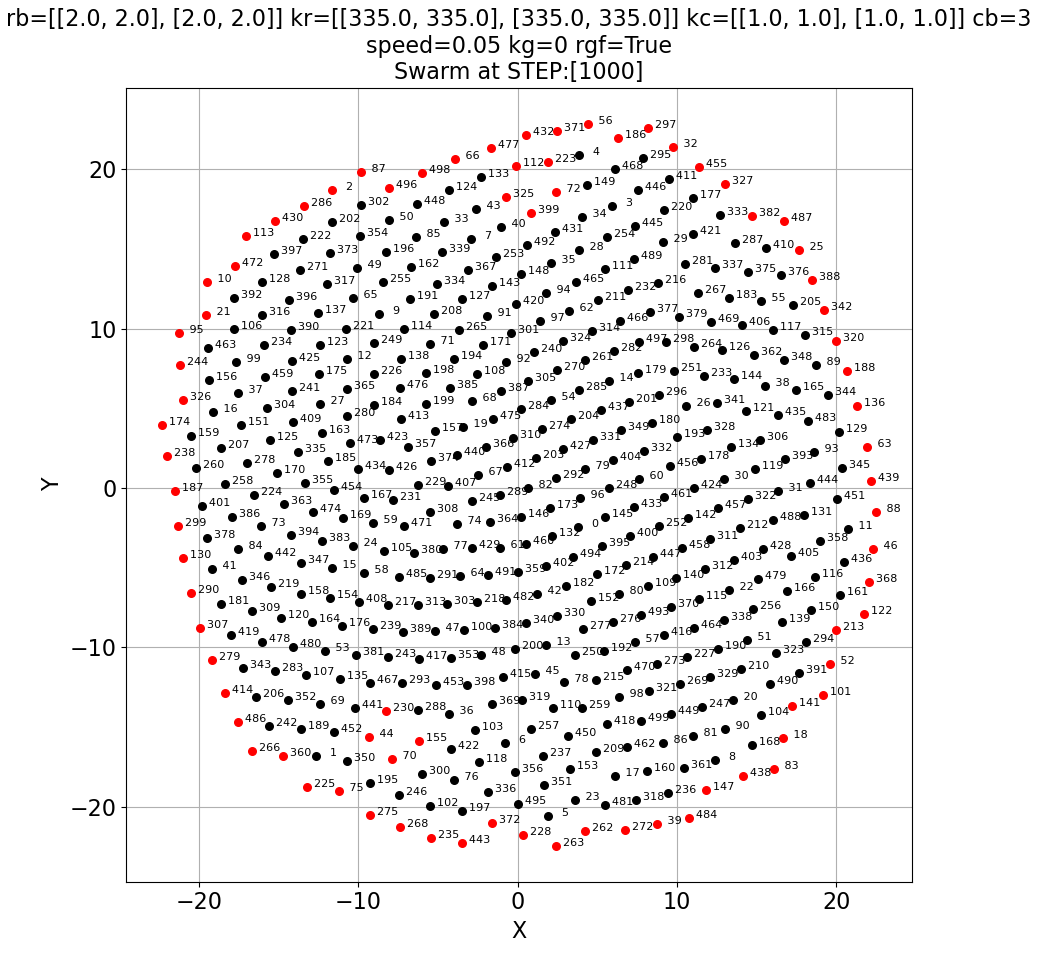
\includegraphics[width=1.0\linewidth]{figures/baseline2-2}
	\end{center}
	\caption{Baseline 2 end. \label{fig:baseline2-2}}
\end{figure}

The Magnitude metric shows that the baseline 2 swarm starts with a high magnitude due to the compression and the swarm. There is also a high degree of `jitter' (Fig.~\ref{fig:baseline2Distance}). However the swarm expands rapidly as can bee seen in the distance metric (Fig.~\ref{fig:baseline2Magnitude}). Over time the magnitude reduces as the swarm expands and the distribution of the agents evening out reducing the internal disruption. Once the swarm has fully expanded at about 400 time steps the swarm settles to is nominal state.

\begin{figure}[H]
	\begin{center}
		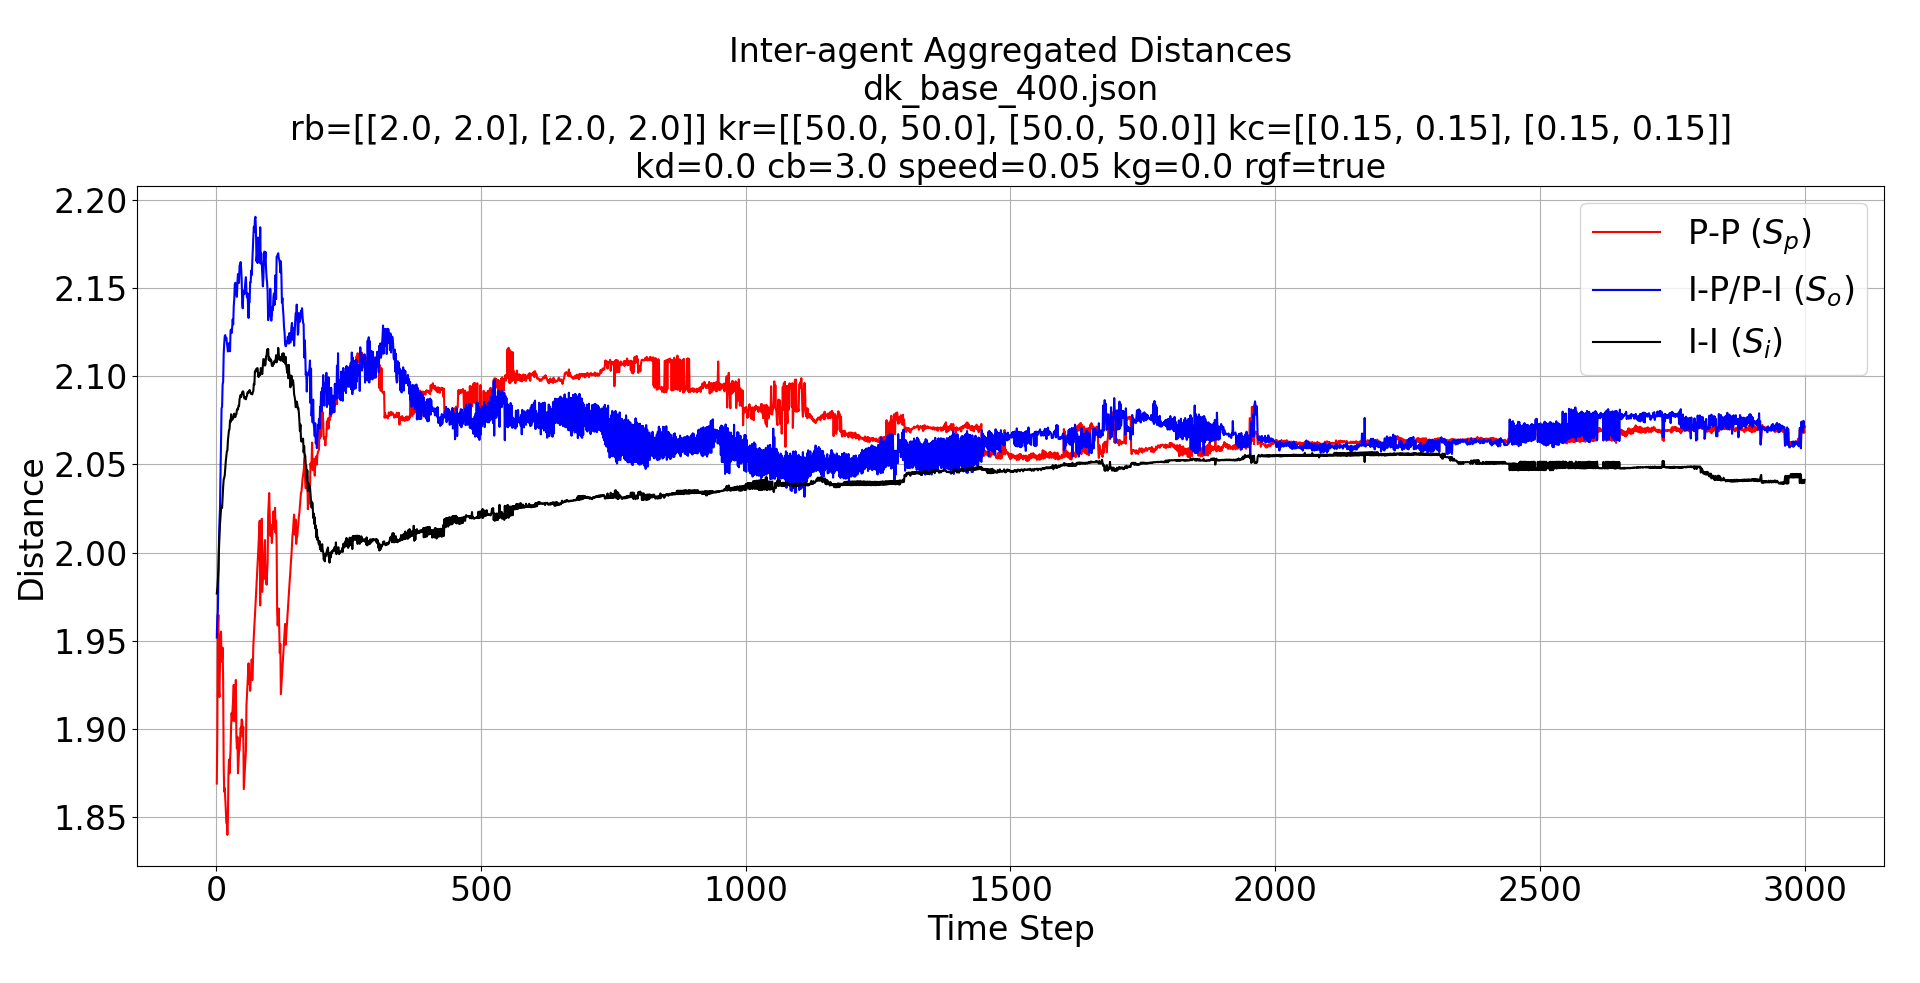
\includegraphics[width=1.0\linewidth]{figures/baseline2Distance}
	\end{center}
	\caption{Baseline 2 (Distance). \label{fig:baseline2Distance}}
\end{figure}

The distance metric (Fig.~\ref{fig:baseline2Distance}) also shows that the swarm settles to a point where the perimeter agents are slightly more dispersed than the internal agents, this is expected due to their constituent vectors being only on the inner side of the swarm. The perimeter\textrightarrow internal agents are slightly closer and the internal\textrightarrow internal agents are distributed more regularly but are slightly closer together due to there being cohesion and repulsion vectors from all sides.

\begin{figure}[H]
	\begin{center}
		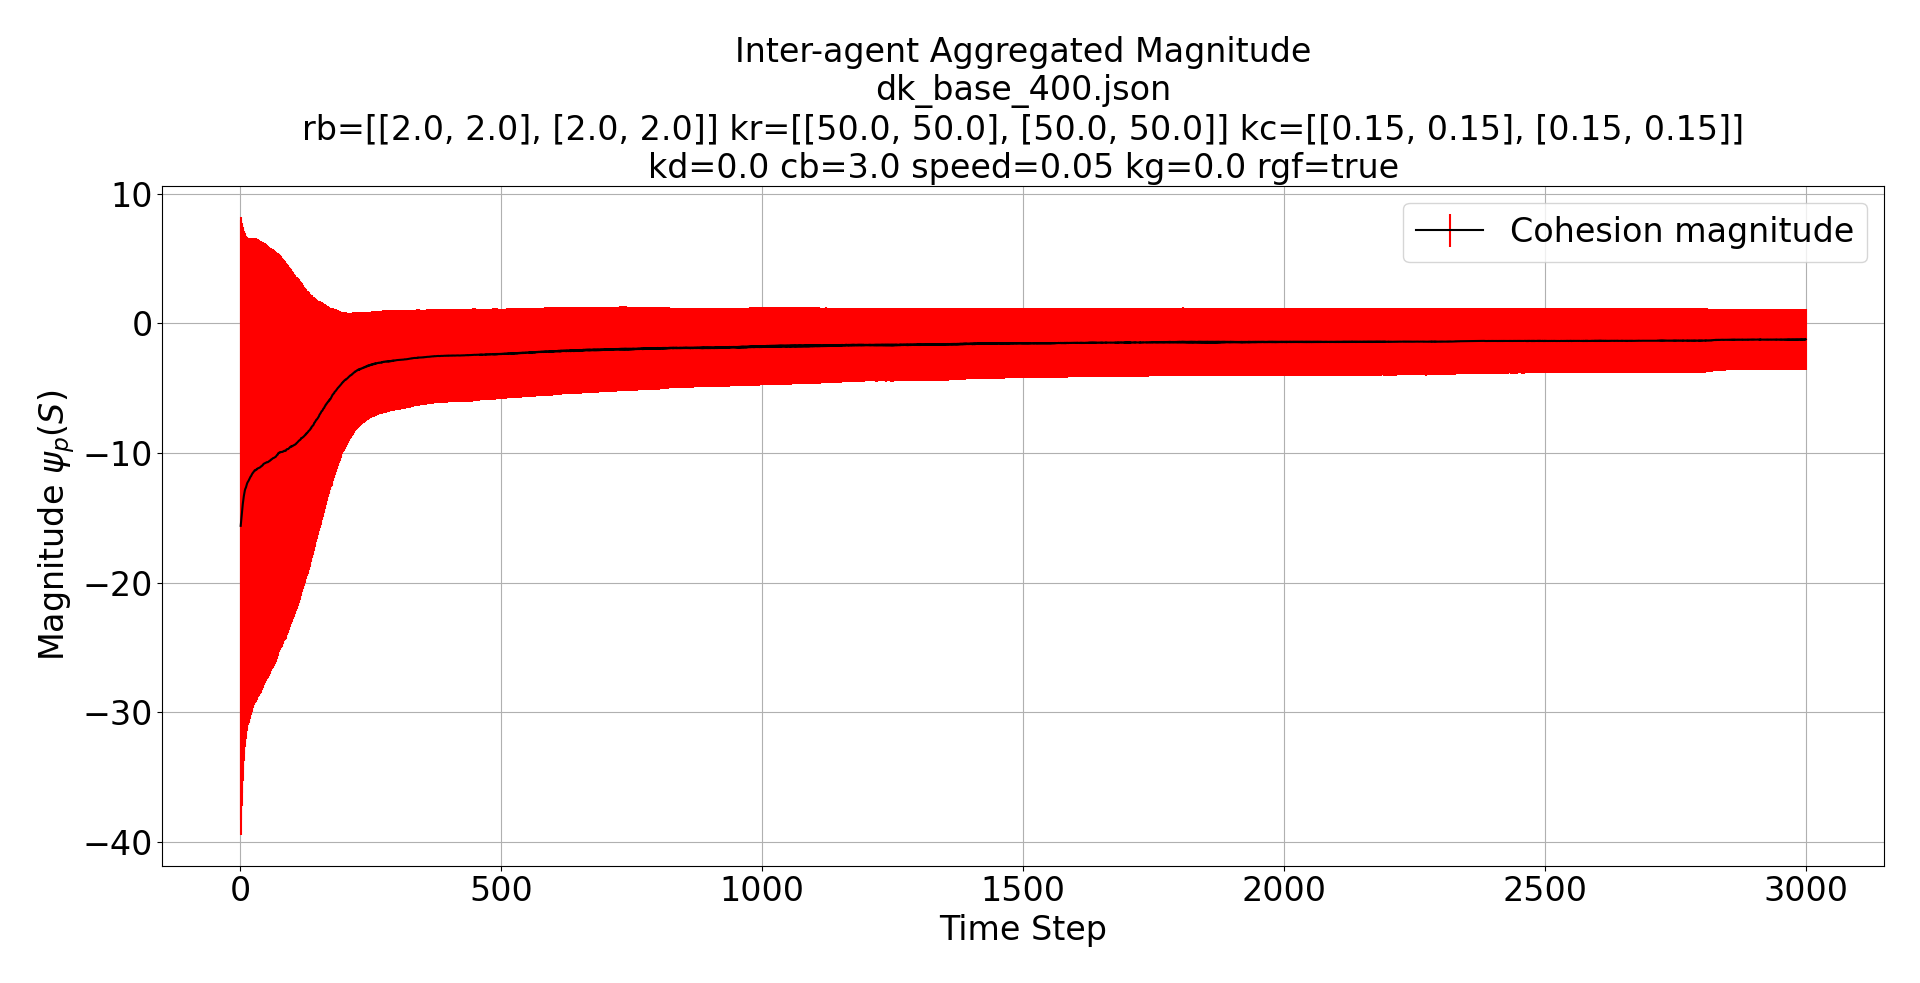
\includegraphics[width=1.0\linewidth]{figures/baseline2Magnitude}
	\end{center}
	\caption{Baseline 2 (Magnitude). \label{fig:baseline2Magnitude}}
\end{figure}


\subsubsection{Perimeter Expansion}
The basis of this experiment is to use the new model to generate a swarm that expands the distance between perimeter-based agents. This would be useful when a swarm is moving into an area that could disable or harm agents to reduce the number of agents and would limit the number of agents that would be lost from the swarm. At the same time the swarm will still need to exhibit a self-healing property.

\begin{equation}\label{eq:rbexp2}
\rb = 
\begin{bmatrix}
2.0 & 2.0\\
2.0 & 2.0
\end{bmatrix}
\end{equation}

\begin{equation}\label{eq:krexp2}
\kr = 
\begin{bmatrix}
50.0 & 335.0\\
50.0 & 50.0
\end{bmatrix}
\end{equation}

\begin{equation}\label{eq:kcexp2}
\kc = 
\begin{bmatrix}
1.0 & 1.0\\
1.0 & 1.0
\end{bmatrix}
\end{equation}

\begin{figure}[H]
	\begin{center}
		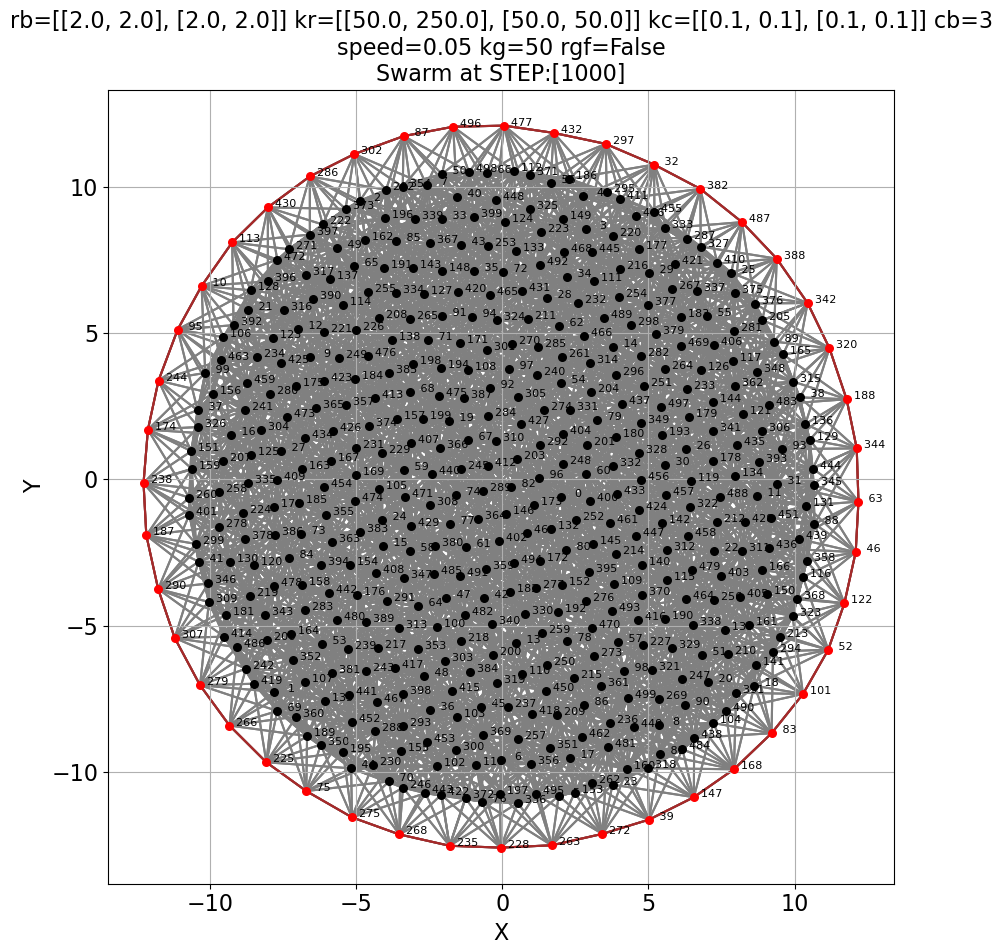
\includegraphics[width=1.0\linewidth]{figures/perimExpand1}
	\end{center}
	\caption{Perimeter Expanded 1. \label{fig:perimExpand1}}
\end{figure}

\begin{figure}[H]
	\begin{center}
		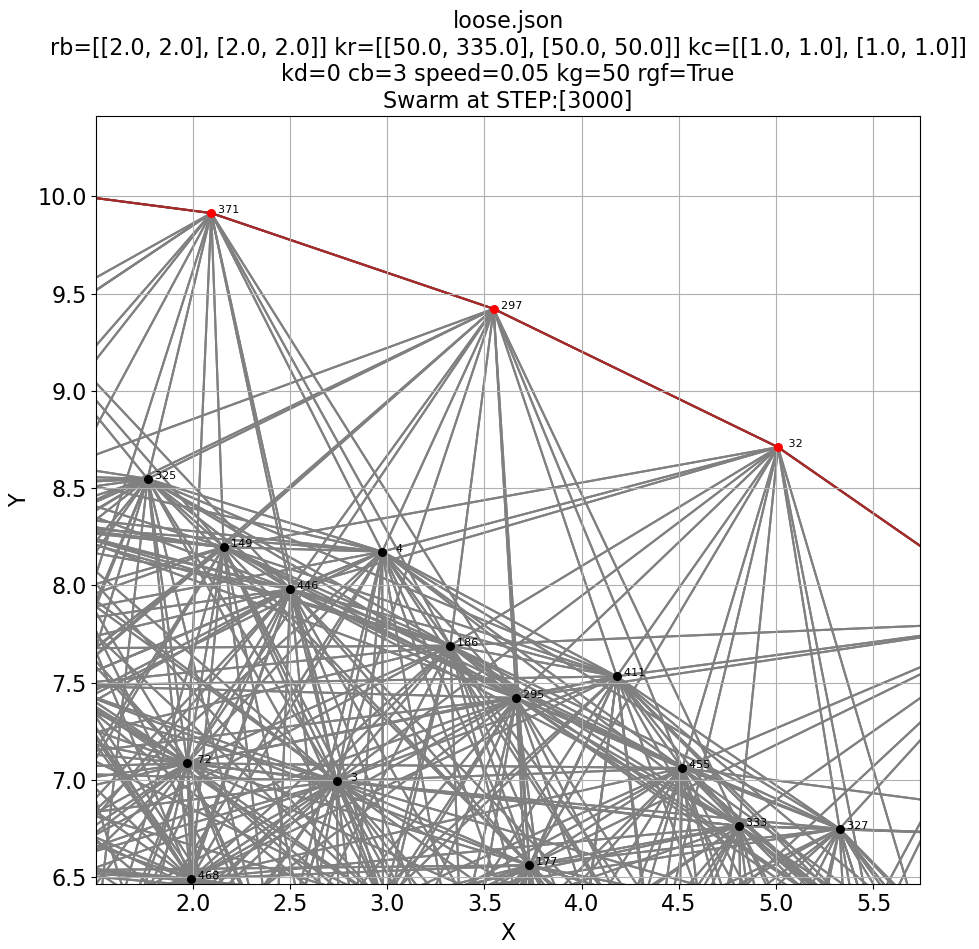
\includegraphics[width=1.0\linewidth]{figures/perimExpand2}
	\end{center}
	\caption{Perimeter Expanded 2. \label{fig:perimExpand2}}
\end{figure}

\begin{figure}[H]
	\begin{center}
		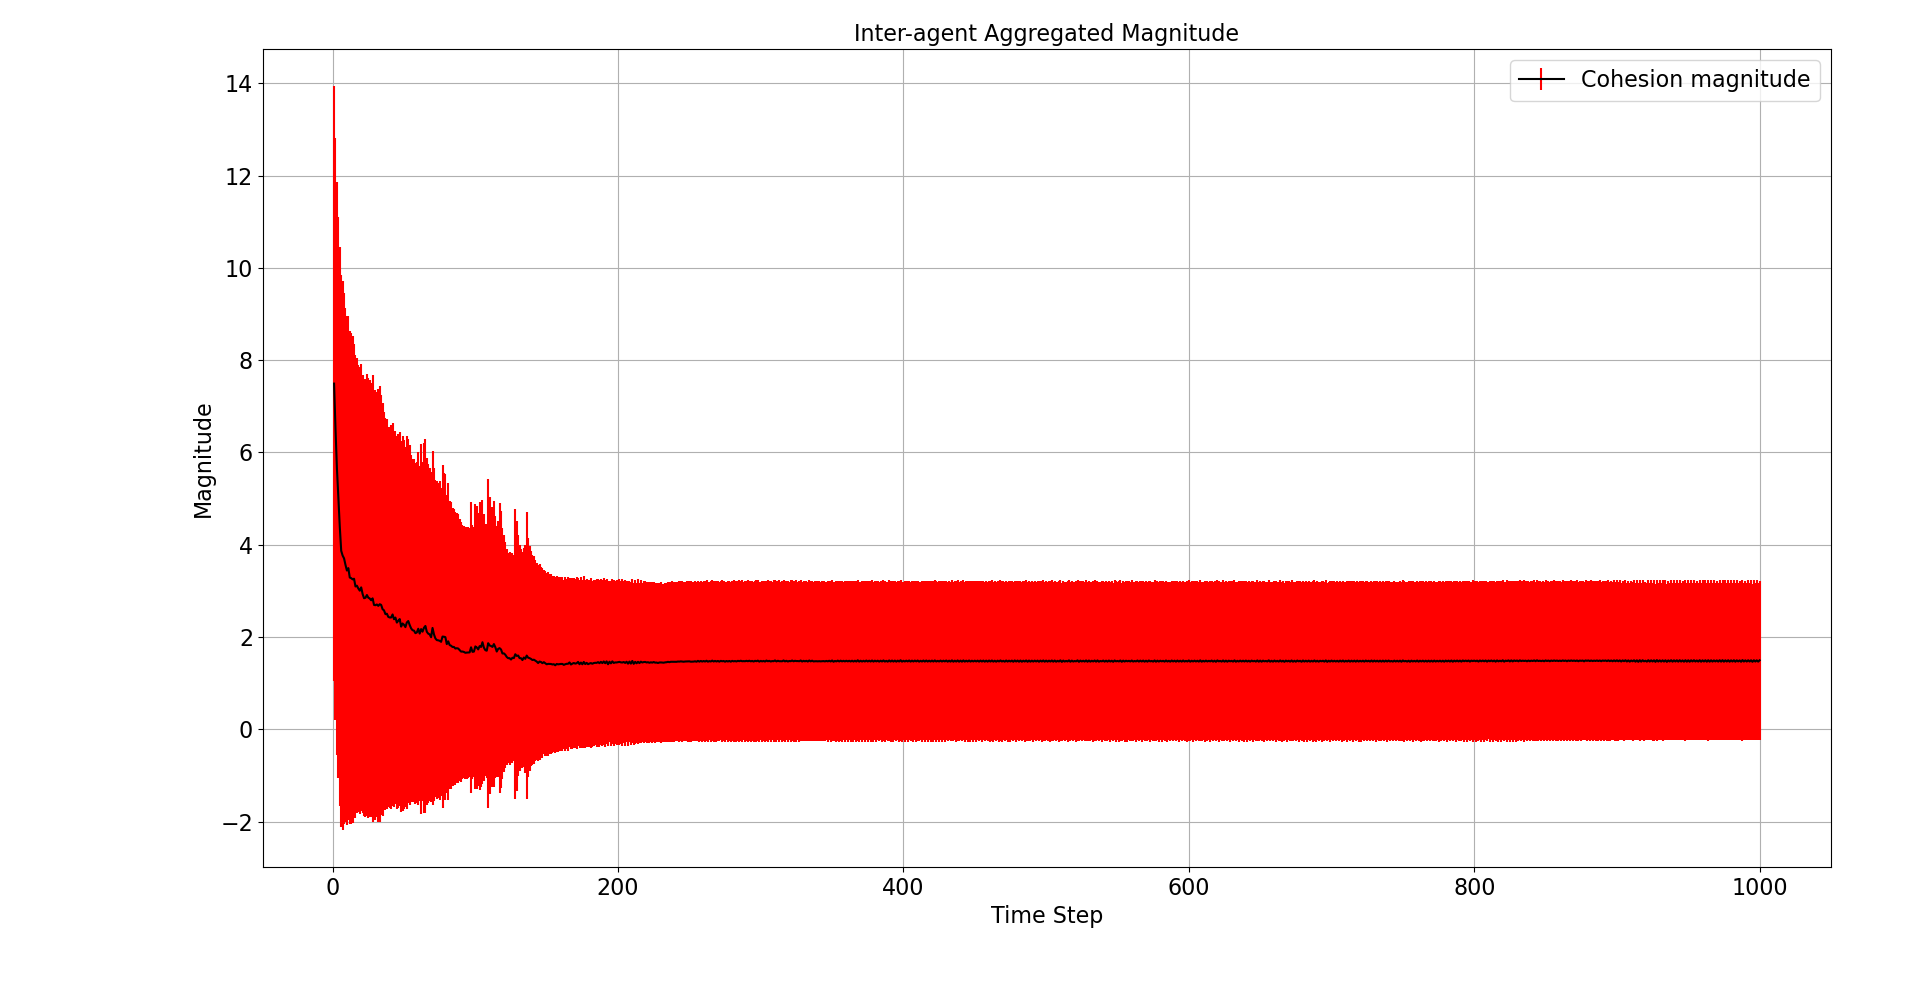
\includegraphics[width=1.0\linewidth]{figures/perimExpandMagnitude}
	\end{center}
	\caption{Perimeter Expanded (Magnitude). \label{fig:perimExpandMagnitude}}
\end{figure}

\begin{figure}[H]
	\begin{center}
		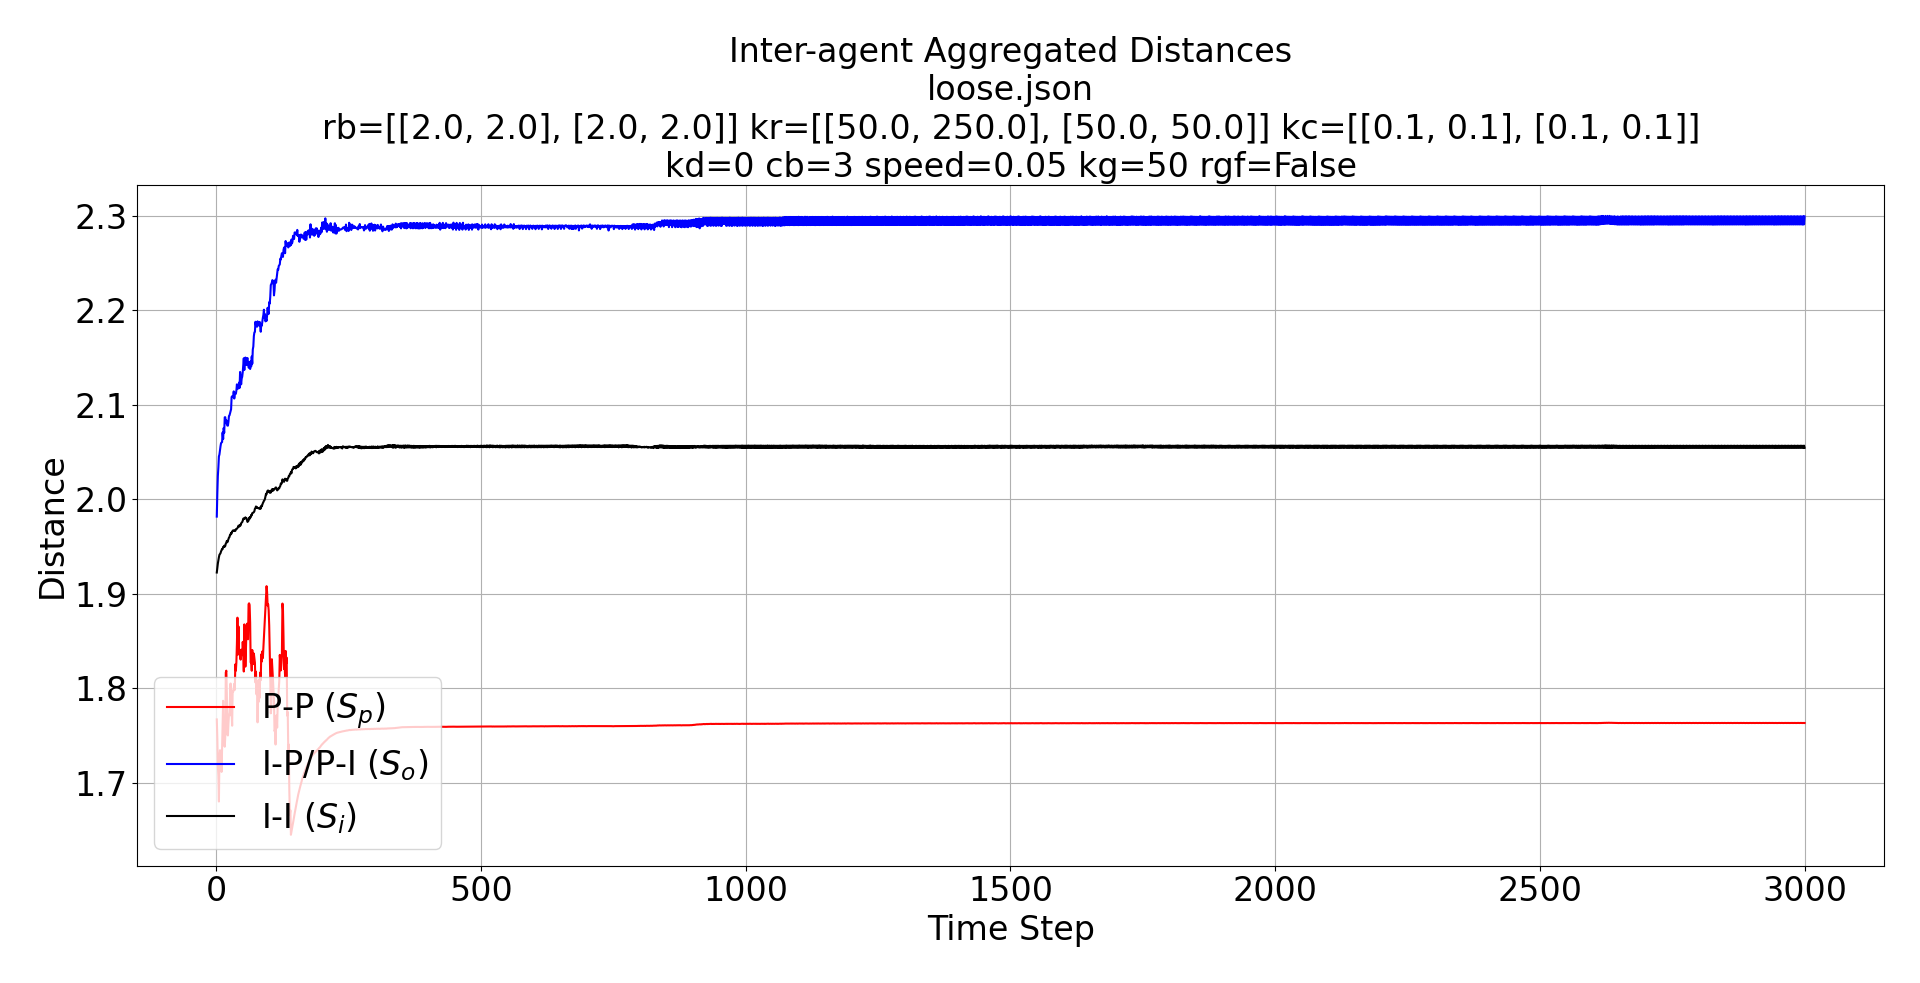
\includegraphics[width=1.0\linewidth]{figures/perimExpandDistance}
	\end{center}
	\caption{Perimeter Expanded (Distance). \label{fig:perimExpandDistance}}
\end{figure}

\begin{figure}[H]
	\begin{center}
		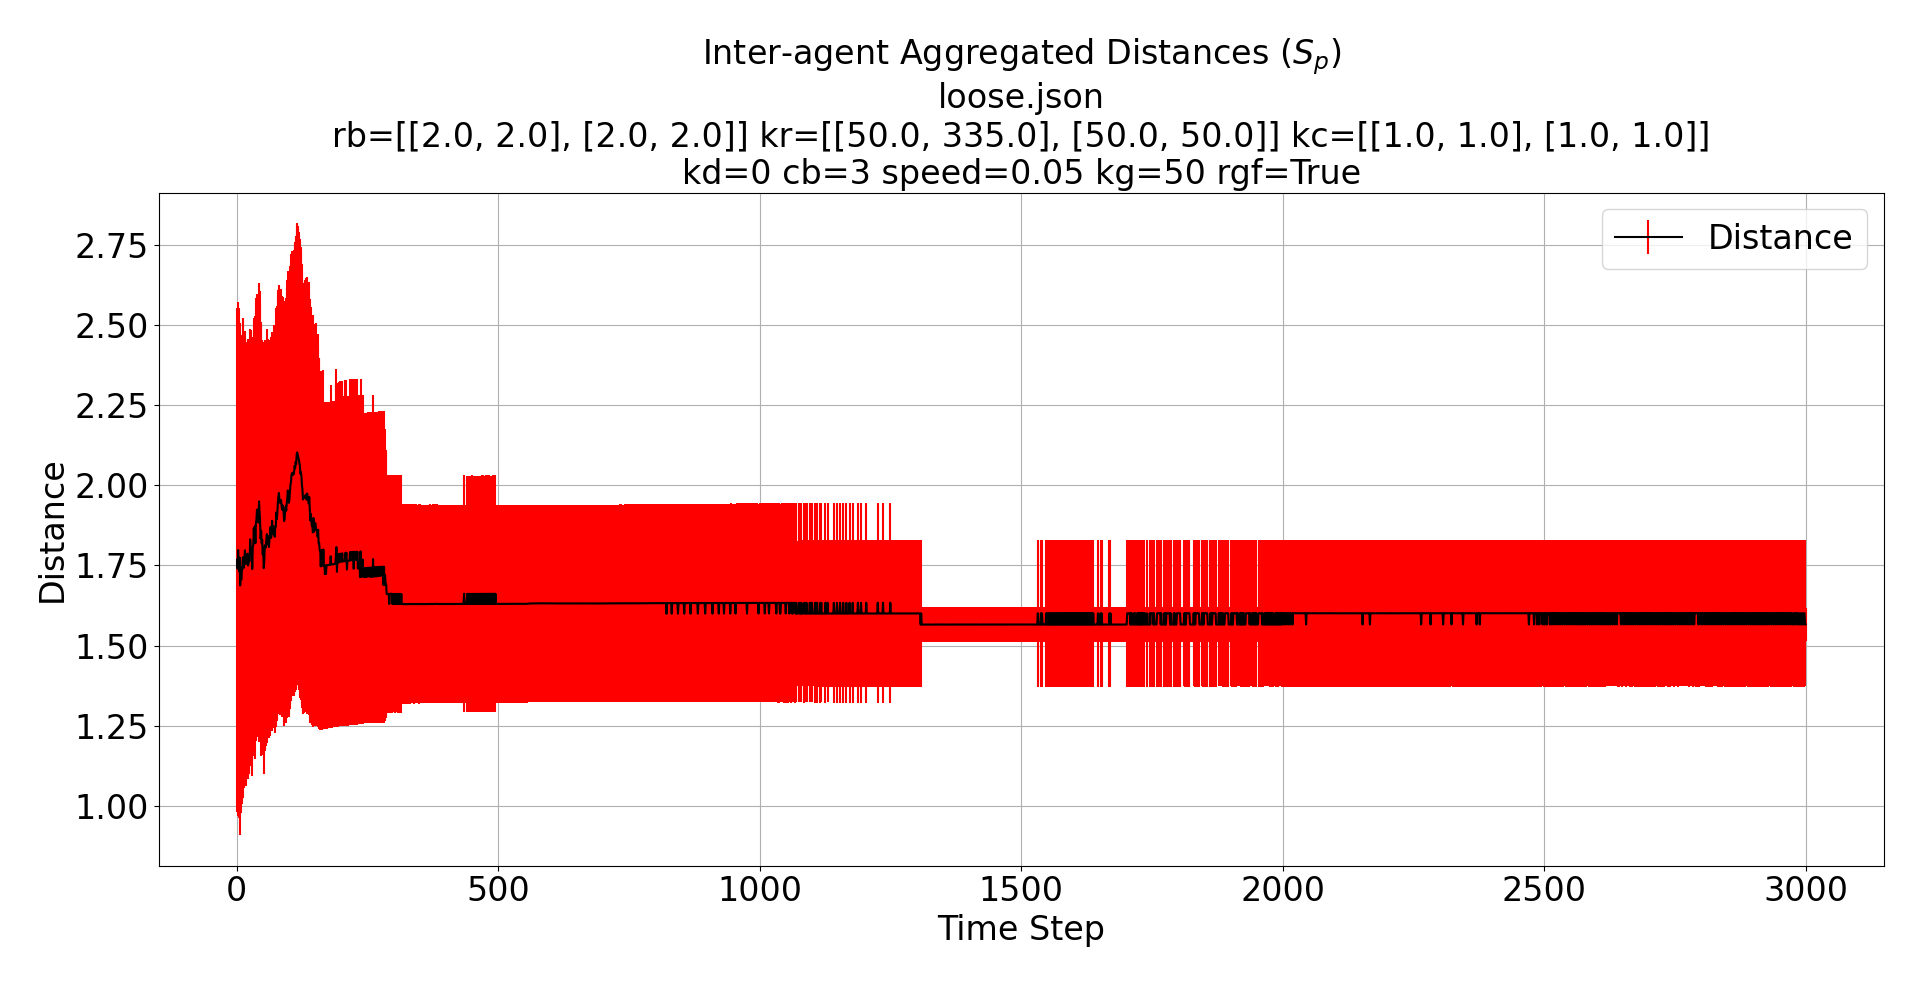
\includegraphics[width=1.0\linewidth]{figures/perimExpandDistancePP}
	\end{center}
	\caption{Perimeter Expanded PP (Distance). \label{fig:perimExpandDistancePP}}
\end{figure}

\begin{figure}[H]
	\begin{center}
		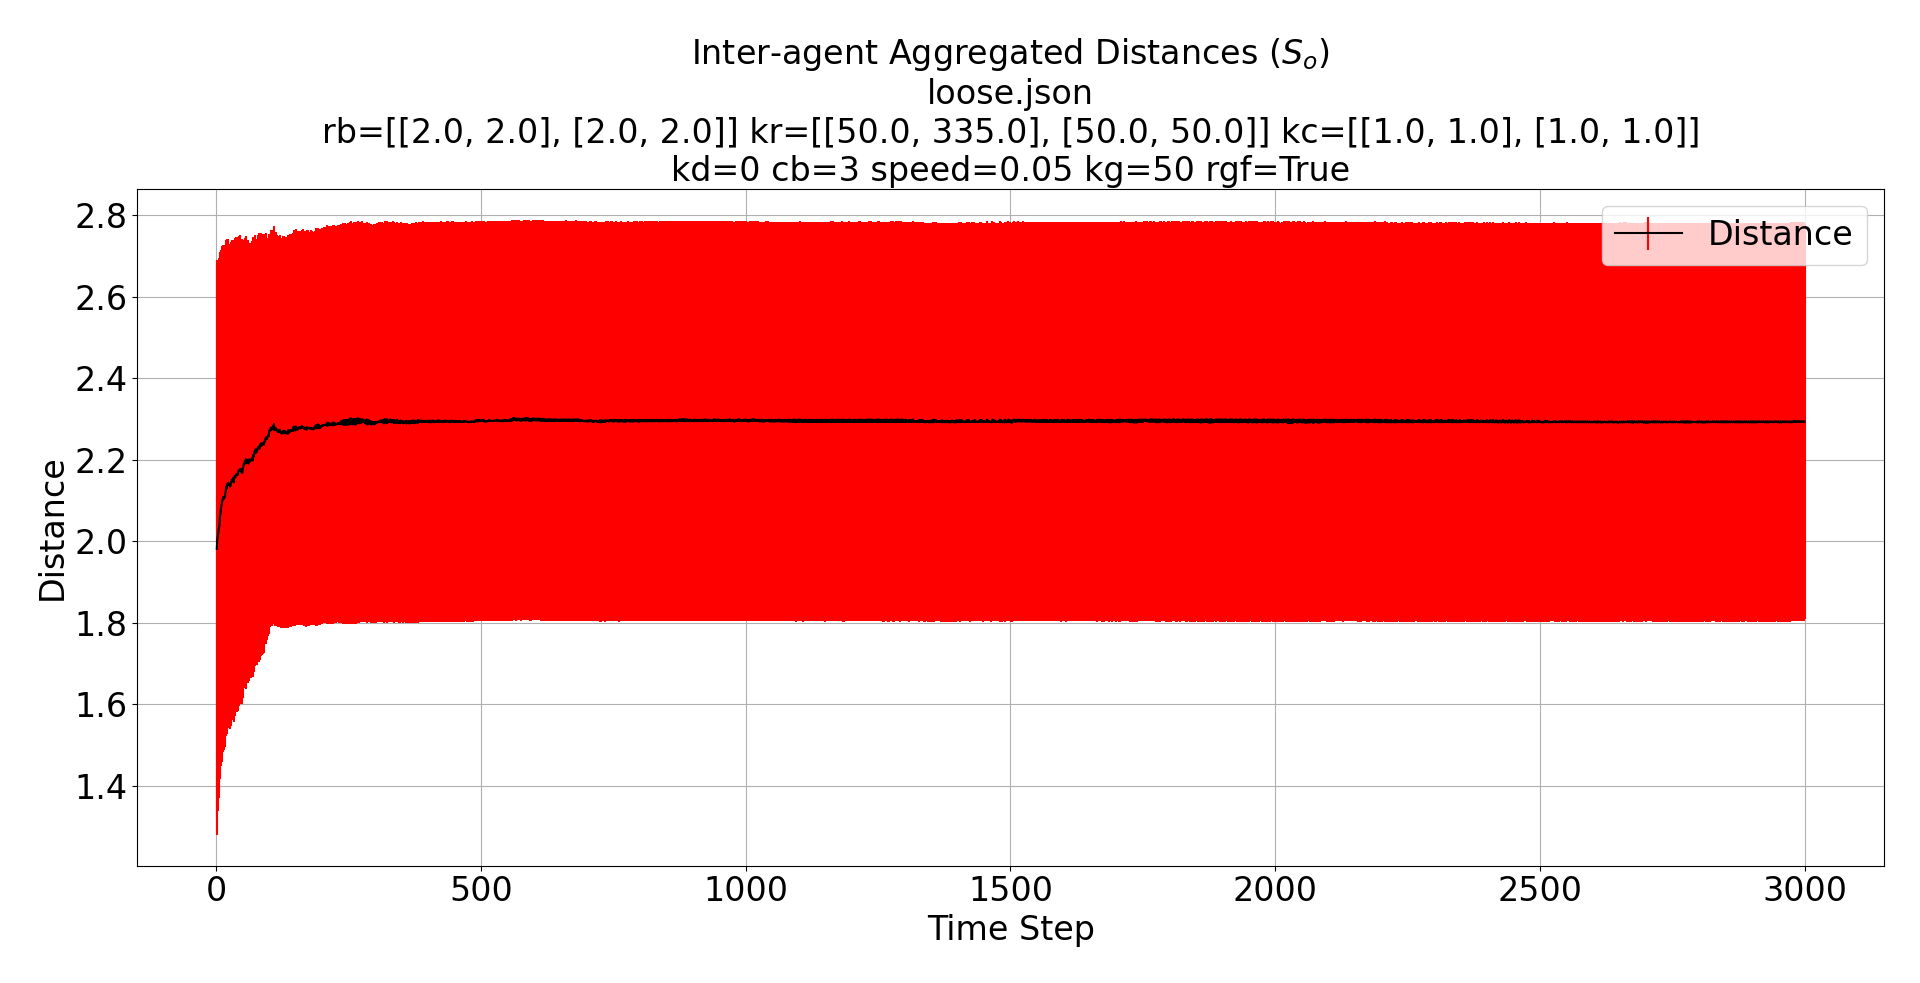
\includegraphics[width=1.0\linewidth]{figures/perimExpandDistanceIPPI}
	\end{center}
	\caption{Perimeter Expanded IPPI (Distance). \label{fig:perimExpandDistanceIPPI}}
\end{figure}

\begin{figure}[H]
	\begin{center}
		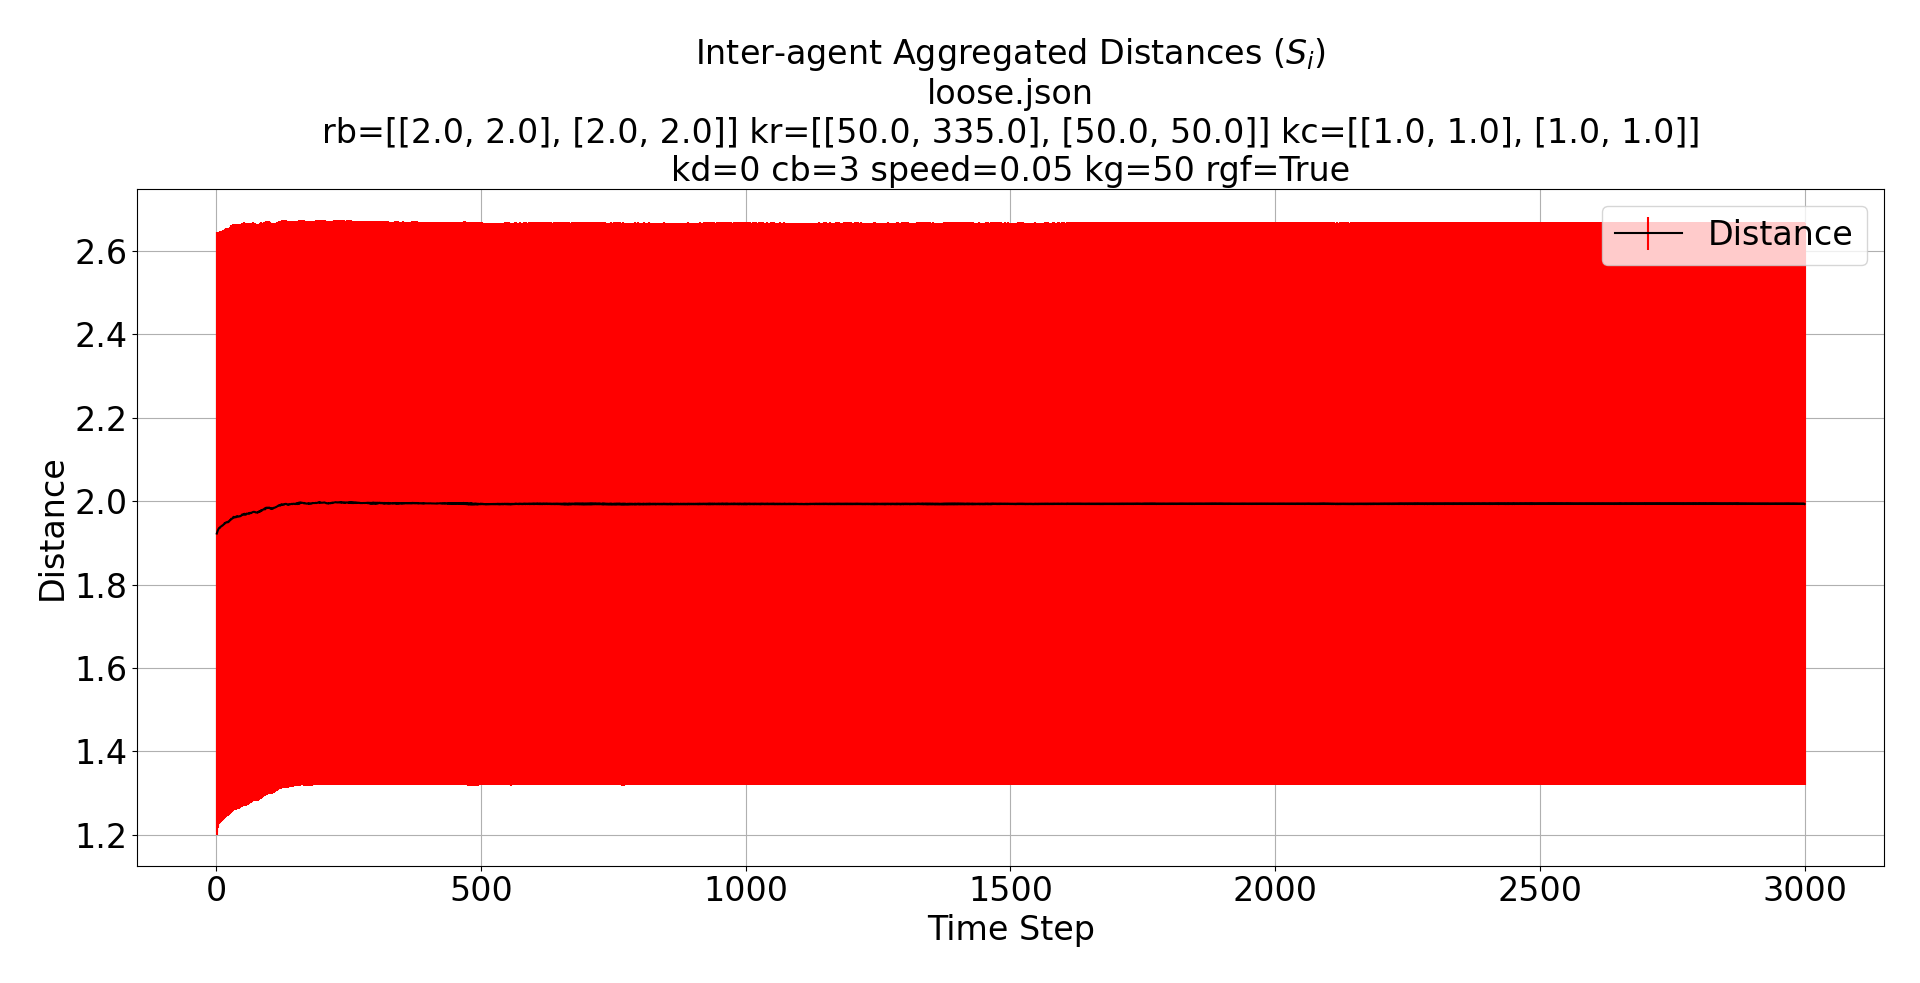
\includegraphics[width=1.0\linewidth]{figures/perimExpandDistanceII}
	\end{center}
	\caption{Perimeter Expanded II (Distance). \label{fig:perimExpandDistanceII}}
\end{figure}


\subsubsection{Packed}

\begin{figure}[H]
	\begin{center}
		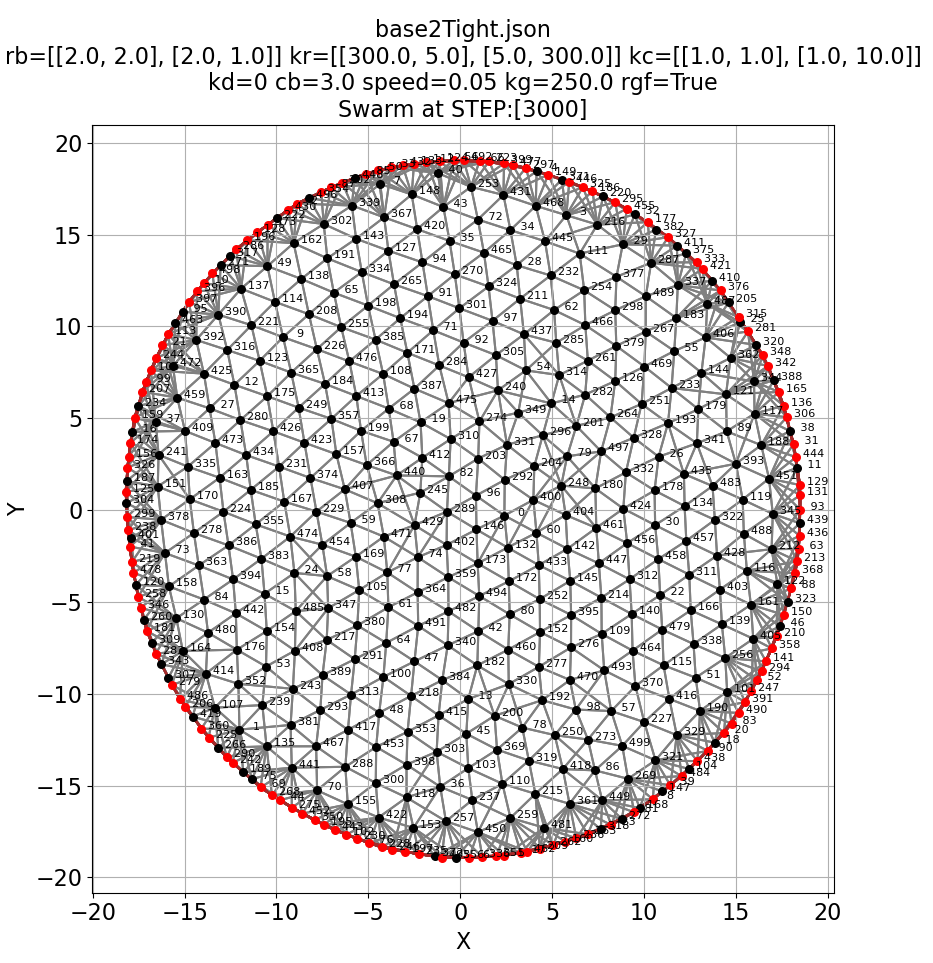
\includegraphics[width=1.0\linewidth]{figures/baseline2Packed}
	\end{center}
	\caption{Perimeter packed\label{fig:perimPackedBaseline2}}
\end{figure}

\begin{figure}[H]
	\begin{center}
		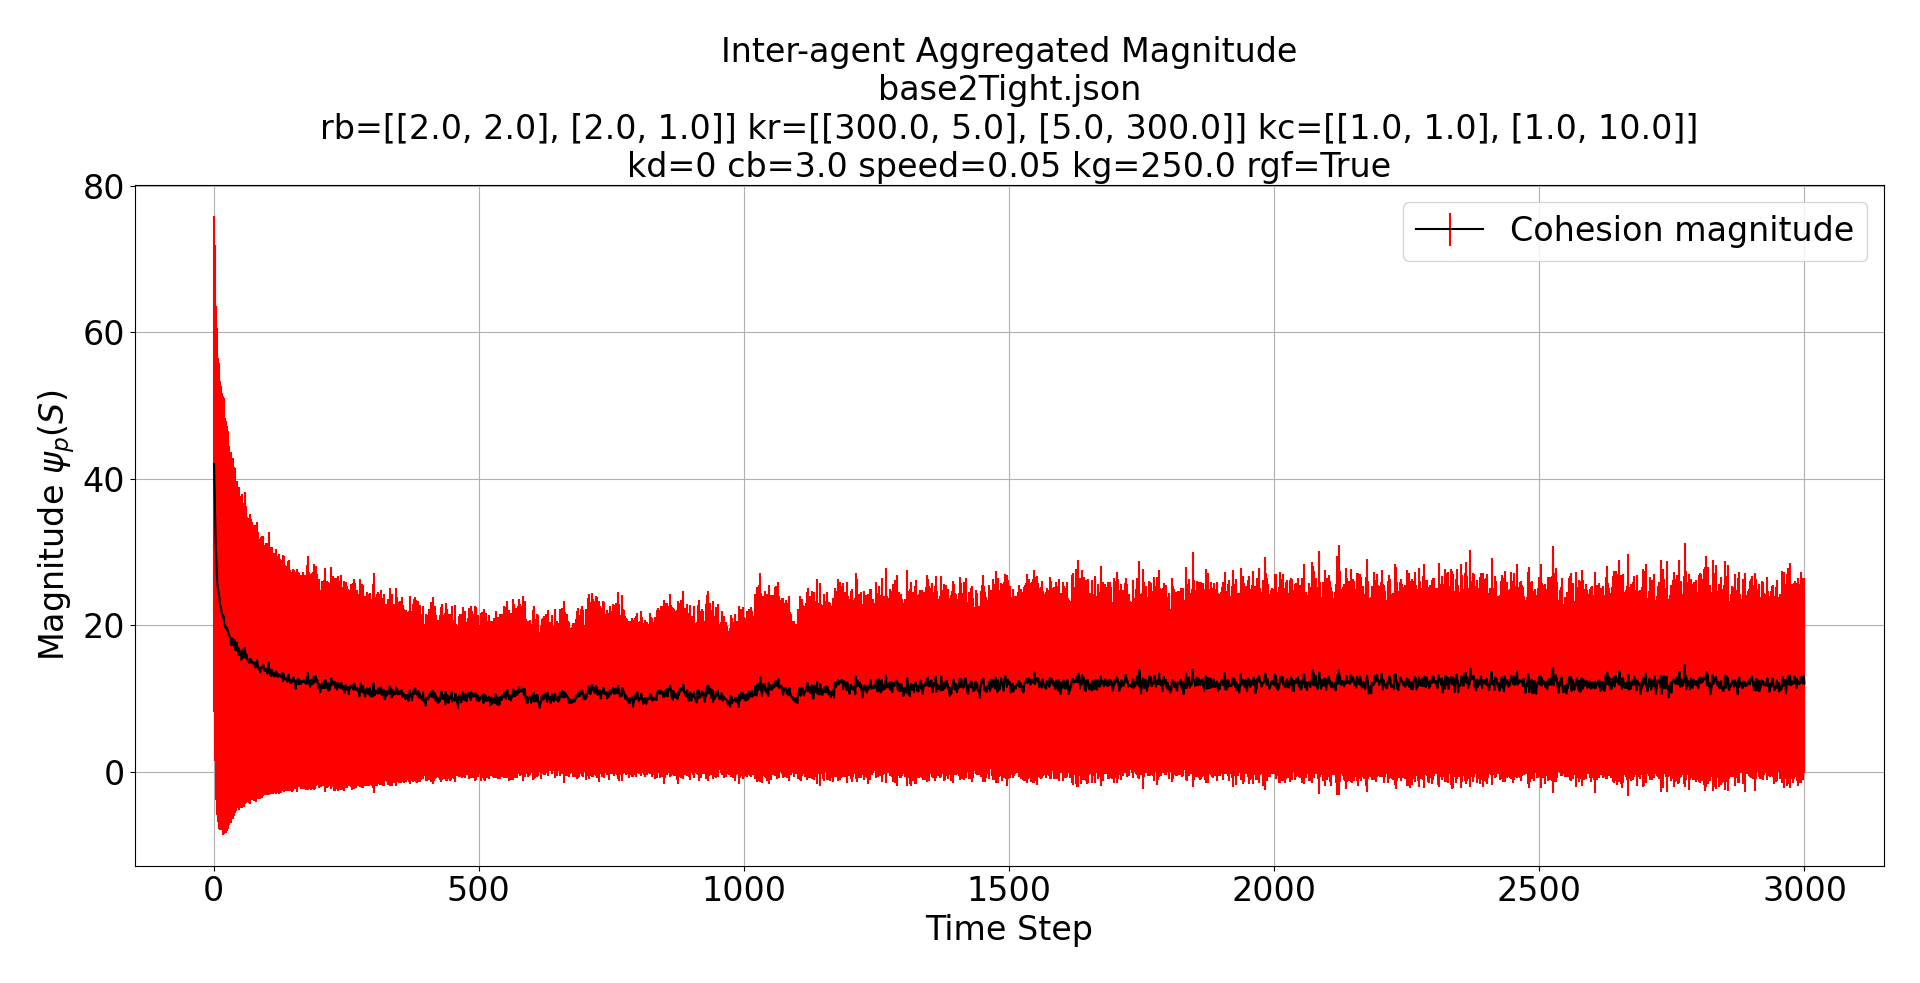
\includegraphics[width=1.0\linewidth]{figures/baseline2PackedMagnitude}
	\end{center}
	\caption{Perimeter packed (Magnitude)\label{fig:baseline2PackedMagnitude}}
\end{figure}

\begin{figure}[H]
	\begin{center}
		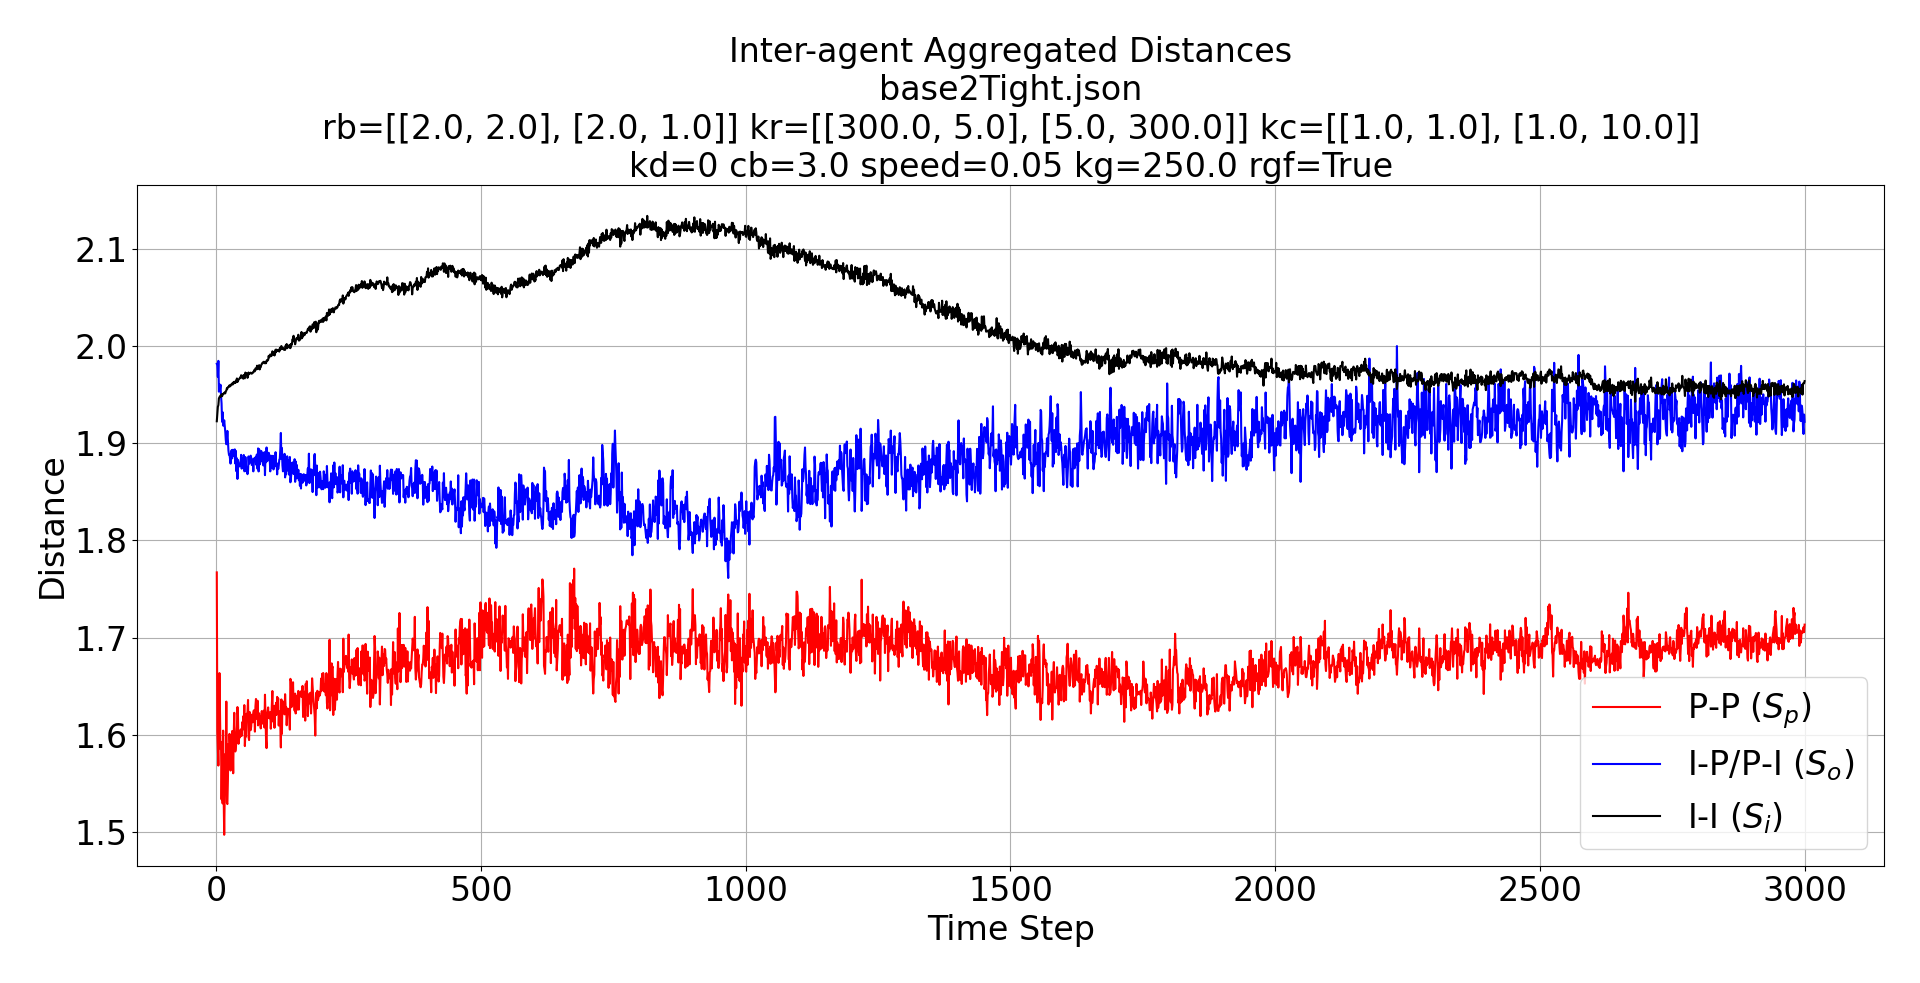
\includegraphics[width=1.0\linewidth]{figures/baseline2PackedDistance}
	\end{center}
	\caption{Perimeter packed (Distance)\label{fig:baseline2PackedDistance}}
\end{figure}

\section{Conclusions and future work}\label{conclusions}
From the initial simulations it is possible to show that the technique is able to successfully restructure swarms into usable configurations based upon the requirements of 4 distinct relationships with the swarm. Also, by adjusting the gap reducing vector to not use the reflex angles it is possible to allow the perimeter agents to circulate around areas that form naturally which requires more analysis to fully realise its potential and application, this effect can be seem in the video located at \url{https://youtu.be/E4Q4hk4KrWA} . Additionally it is possible to remove voids and therefore surround an obstacles. The metrics show that the algorithms do have an impact on swarm stability to exhibit these new features but the impact is consistent throughout the swarms lifetime as it migrates into different structures.

Going forward the new model will be examined based upon the introduction of direction and obstacles. Initial testing shows that the models holds up well including the improvement in self-healing as demonstrated in figure~\ref{fig:packedSelfHealing} which demonstrates an obstacle being introduced and removed in a packed perimeter swarm. Figure~\ref{fig:future7} shows the impact on the Magnitude and figure~\ref{fig:future8} shows the impact on the inter-agent distances.
\begin{figure*}[ht!]
  \begin{center}
    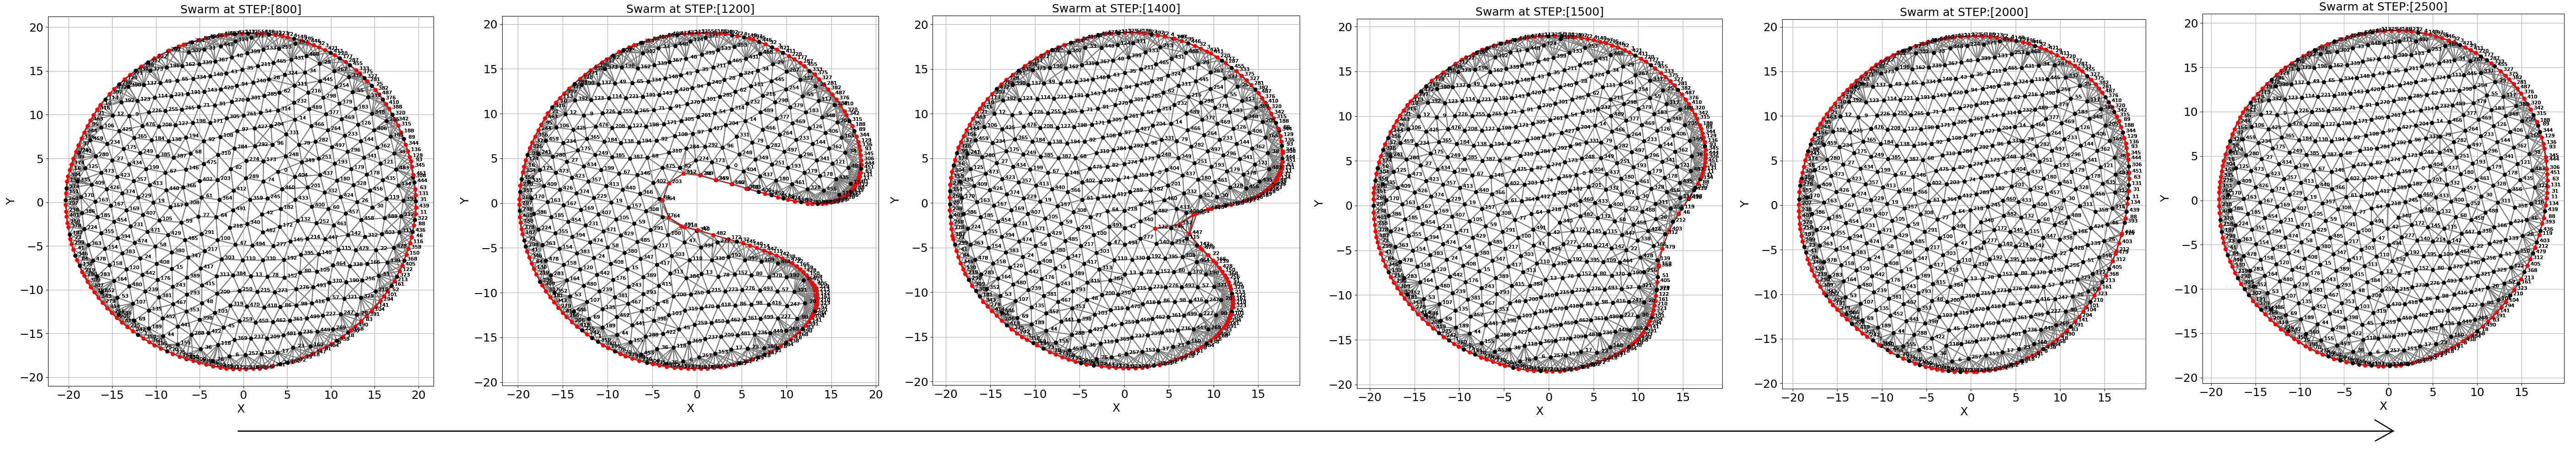
\includegraphics[width=17.6cm]{figures/FutureTime}
  \end{center}
  \caption{Simulation of a packed perimeter demonstrating self-healing properties over time\label{fig:packedSelfHealing}}
\end{figure*}

\begin{figure}[H]
	\begin{center}
		\includegraphics[width=1.0\linewidth]{figures/future7}
	\end{center}
	\caption{Perimeter packed (Magnitude)\label{fig:future7}}
\end{figure}

\begin{figure}[H]
	\begin{center}
		\includegraphics[width=1.0\linewidth]{figures/future8}
	\end{center}
	\caption{Perimeter packed (Distance)\label{fig:future8}}
\end{figure}

\bibliographystyle{abbrv}
\bibliography{perimeter}

\end{document}